% -*- root: ../main.tex -*-

% In questa sezione esporre brevemente i requisiti a cui il sistema proposto deve rispondere, concentrando l'attenzione sugli aspetti più rilevanti e facendo eventualmente uso di opportuni diagrammi di alto livello.
% 8000 - 10000 battute
% Attenzione in particolare ai requirement non funzionali: 1) non siano troppo vaghi altrimenti sono inverificabili, e quindi praticamente inutili; 2) se il sistema è distribuito, è inevitable dire cosa vi aspettate in termini di di robustezza a cambiamenti/guasti (quali?, come?), e scalabilità (in quale dimensione? fino a che punto?).

\chapter{Analisi dei Requisiti}
A seguito dell'intervista con l'esperto del dominio, sono emersi i seguenti requisiti per l'applicativo richiesto. Questi sono stati poi discussi e approvati dal committente.
\section{Requisiti di Business}
    L'importanza strategica del software risiede nel fornire agli studenti un valido strumento di ripasso e test delle competenze acquisite.
    Le aree semantiche di maggiore importanza sono l'interrogazione delle conoscenze tramite quesiti, il feedback sugli errori, la personalizzazione dei quiz, le statistiche globali e il riepilogo a fine partita. 
    I principali punti sono sotto riportati:
    \begin{itemize}
        \item selezione di N domande tra i C corsi scelti dell'utente
        \item gestione delle domande e delle relative risposte permettendo l'editing, il salvataggio e il caricamento delle stesse
        \item elaborare un riepilogo al termine di ogni partita
        \item elaborare e salvare alcune statistiche di interesse relativamente ad un utente
    \end{itemize}
	
\section{Requisiti Utente}
    Uno utente dell'applicazione dovrà quindi essere in grado di:
    \begin{itemize}
        \item ripassare: visualizzare domande e scegliere tra le possibili risposte
        \item scegliere tra varie modalità di gioco
        \item visualizzare un riepilogo a fine partita
        \item visualizzare le proprie statistiche su tutte le partite effettuate
        \item importare ed esportare nuovi quiz, con le relative domande e risposte
    \end{itemize}
 
        \subsection{User Stories}
        \label{chap:UserStories}
        Si riportano di seguito le user stories emerse:
        \begin{enumerate}
            \item \label{us:inizio-partita} come utente voglio poter accedere all'applicativo e iniziare una nuova partita
            \item \label{us:selezione-e-feedback} come utente voglio poter selezionare la risposta che ritengo corretta, ricevendo un feedback a riguardo
            \item \label{us:revisione-quiz} come utente voglio poter riguardare i quiz della partita appena terminata
            \item \label{us:visione-statistiche} come utente voglio poter visualizzare le mie statistiche personali
            \item \label{us:selezione-corsi} come utente voglio poter selezionare i corsi prima dell'inizio di ogni partita
            \item \label{us:selezione-modalità} come utente voglio poter selezionare la modalità di gioco
            \item \label{us:impostazioni} come utente voglio poter cambiare le impostazioni di gioco
            \item \label{us:aggiunta-quiz} come utente voglio poter aggiungere dei quiz, qualora ne volessi integrare dei nuovi
            \item \label{us:modifica-quiz} come utente voglio poter modificare i quiz aggiunti, qualora non siano corretti
            \item \label{us:aggiunta-corso} come utente voglio poter aggiungere dei corsi, qualora ne volessi integrare dei nuovi
            \item \label{us:modifica-corso} come utente voglio poter modificare i corsi già presenti, qualora non siano corretti
            \item \label{us:importa-quiz} come utente voglio poter importare i quiz in blocco relativi a uno o più corsi
            \item \label{us:esporta-quiz} come utente voglio poter esportare i quiz in blocco relativi a uno o più corsi
        \end{enumerate}
        
        \begin{figure}[H]
            \centering
            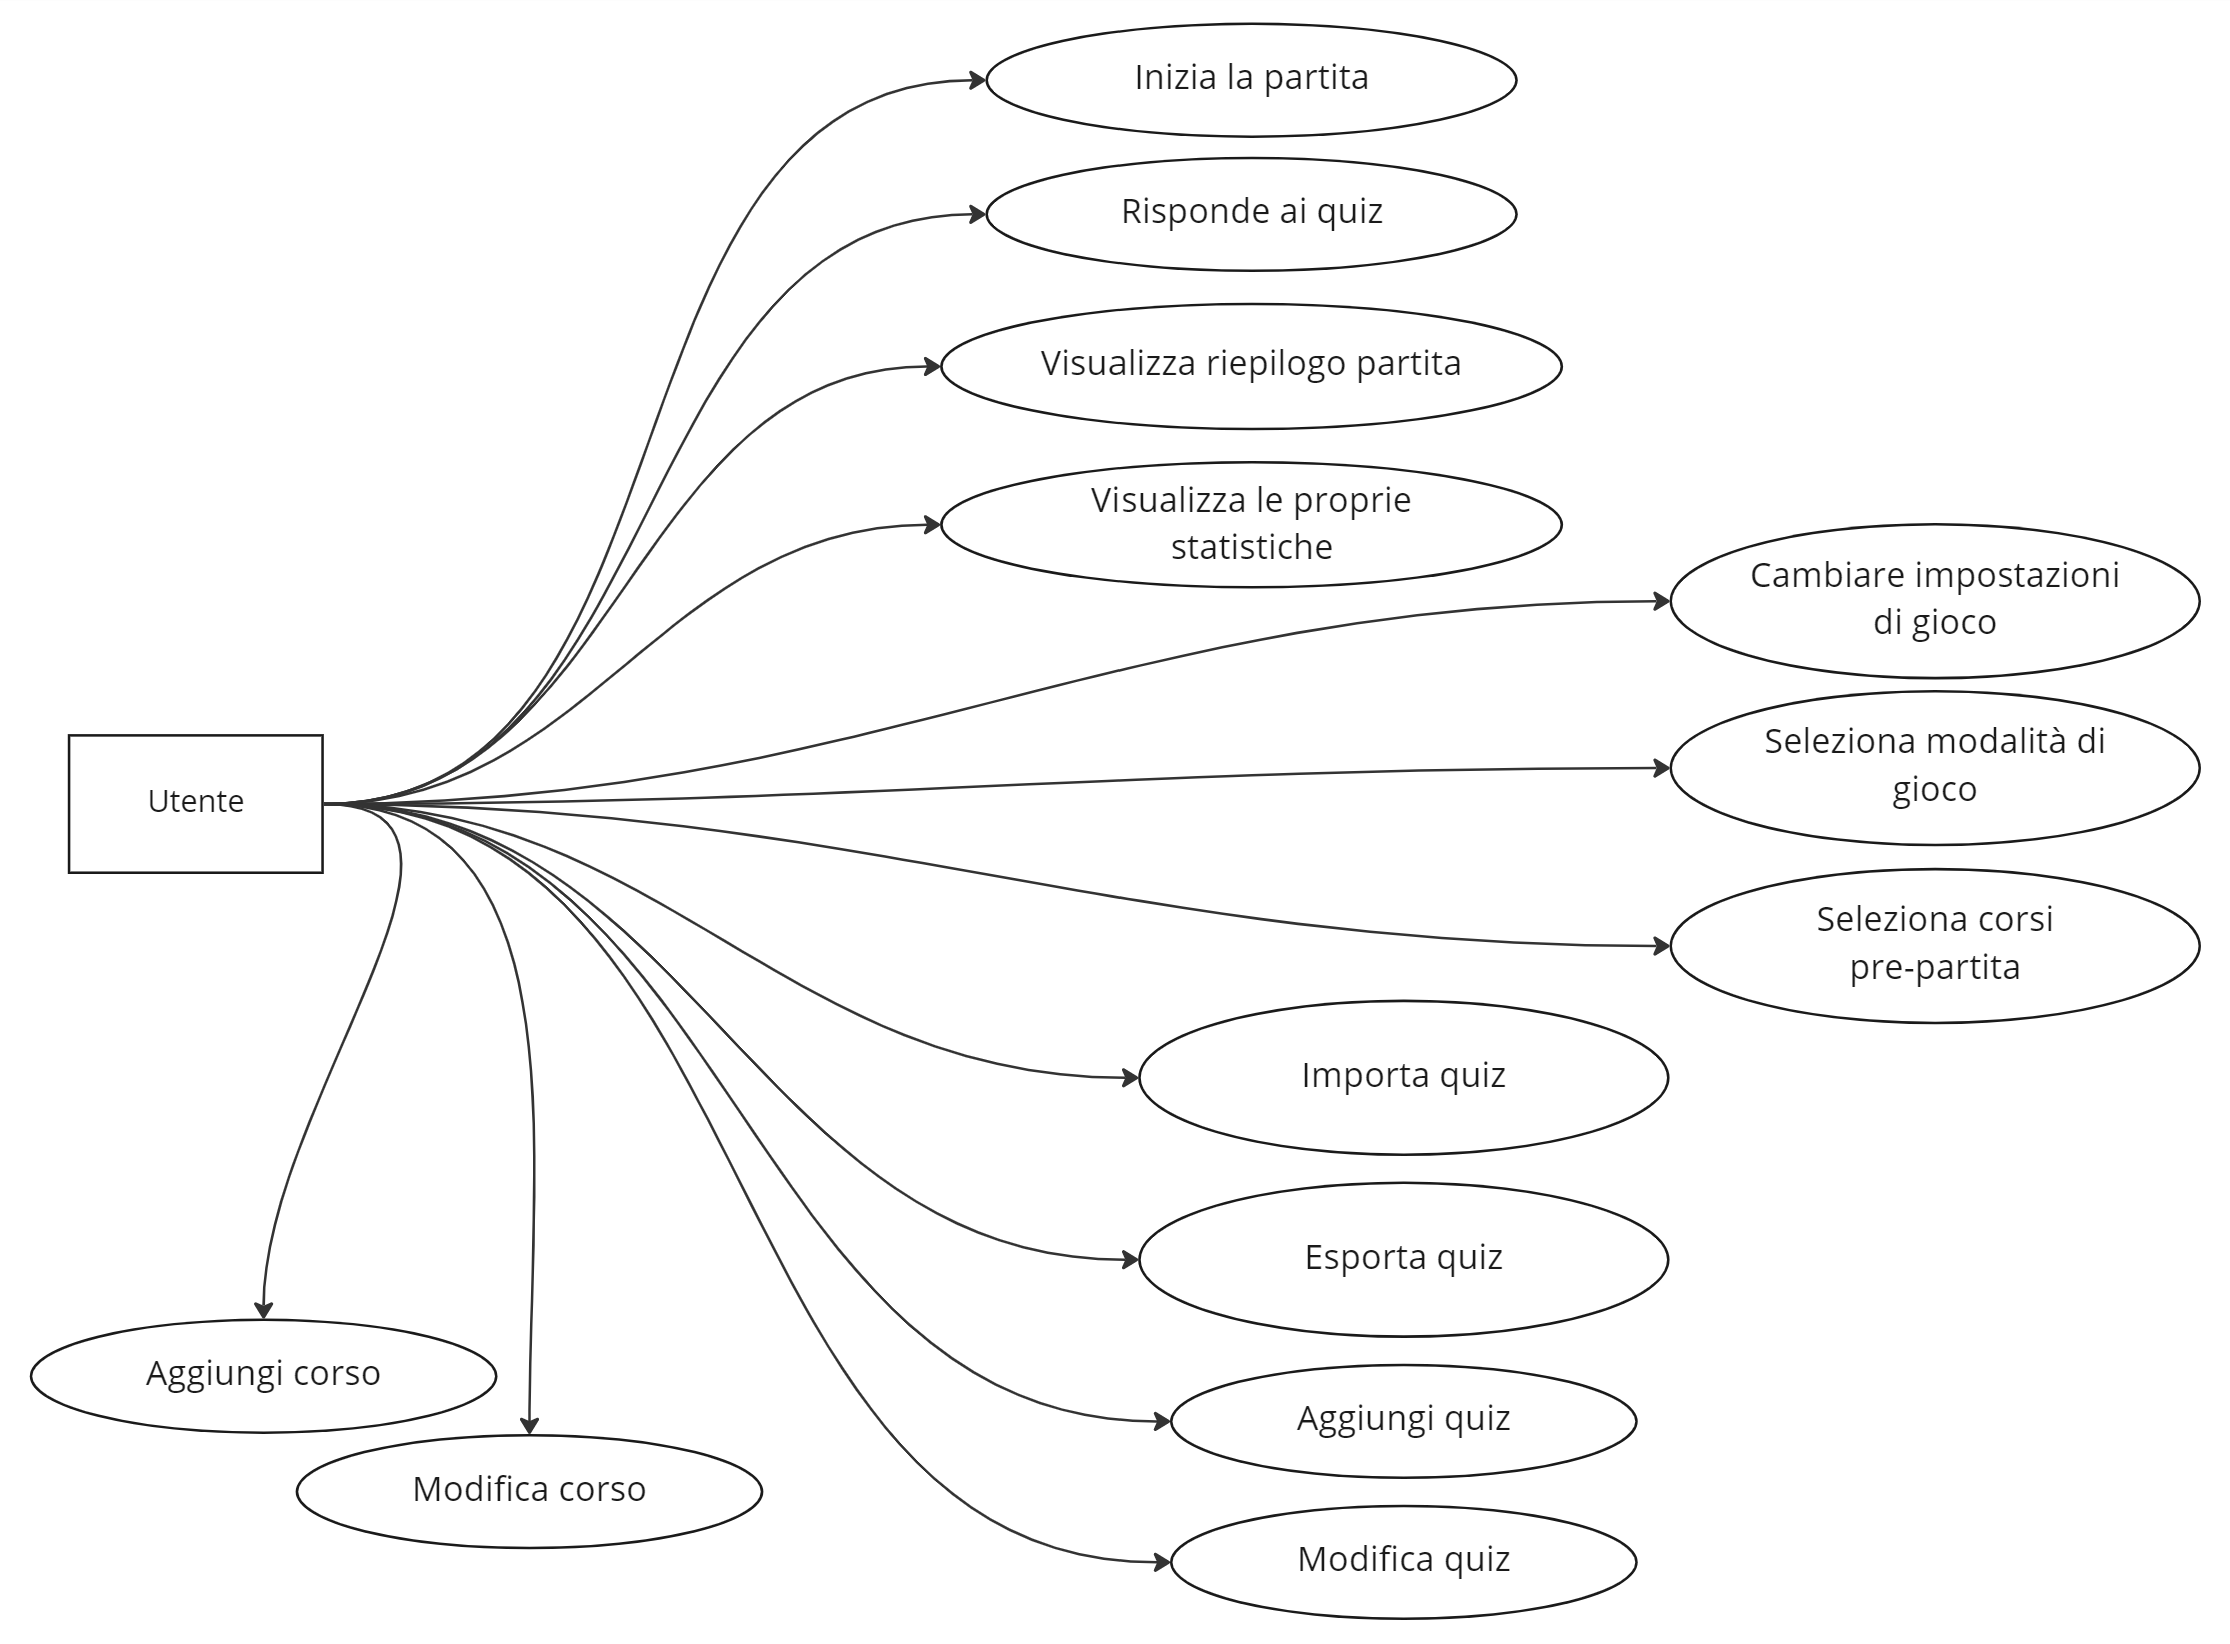
\includegraphics[width=\textwidth]{Miro/use_case.png}
            \caption{Schema Casi d'Uso}
            \label{fig:use-case}
        \end{figure}

        \subsection{Mockup}
        \label{chap:Mockup}
    	A seguito dell'intervista fatta con l'esperto del dominio e dei requisiti raccolti con esso, il team di sviluppo ha prodotto due versioni di mockup (\ref{mockup1} e \ref{mockup2}). In seguito, questi sono stati sottoposti al committente, il quale ha riscontrato aspetti positivi e negativi in entrambe le proposte. Di conseguenza, i mockup definitivi \ref{mockupFinished} sono stati sviluppati con la sua collaborazione e supervisione. Per garantire una maggior comprensione della navigazione all'interno dell'applicativo, è stato prodotto lo schema \ref{fig:mockup_nav}.
     
        \subsubsection{Mockup prima versione}\label{mockup1}
        
        \begin{figure}[H]
          \centering
          \begin{minipage}[b]{0.48\textwidth}
            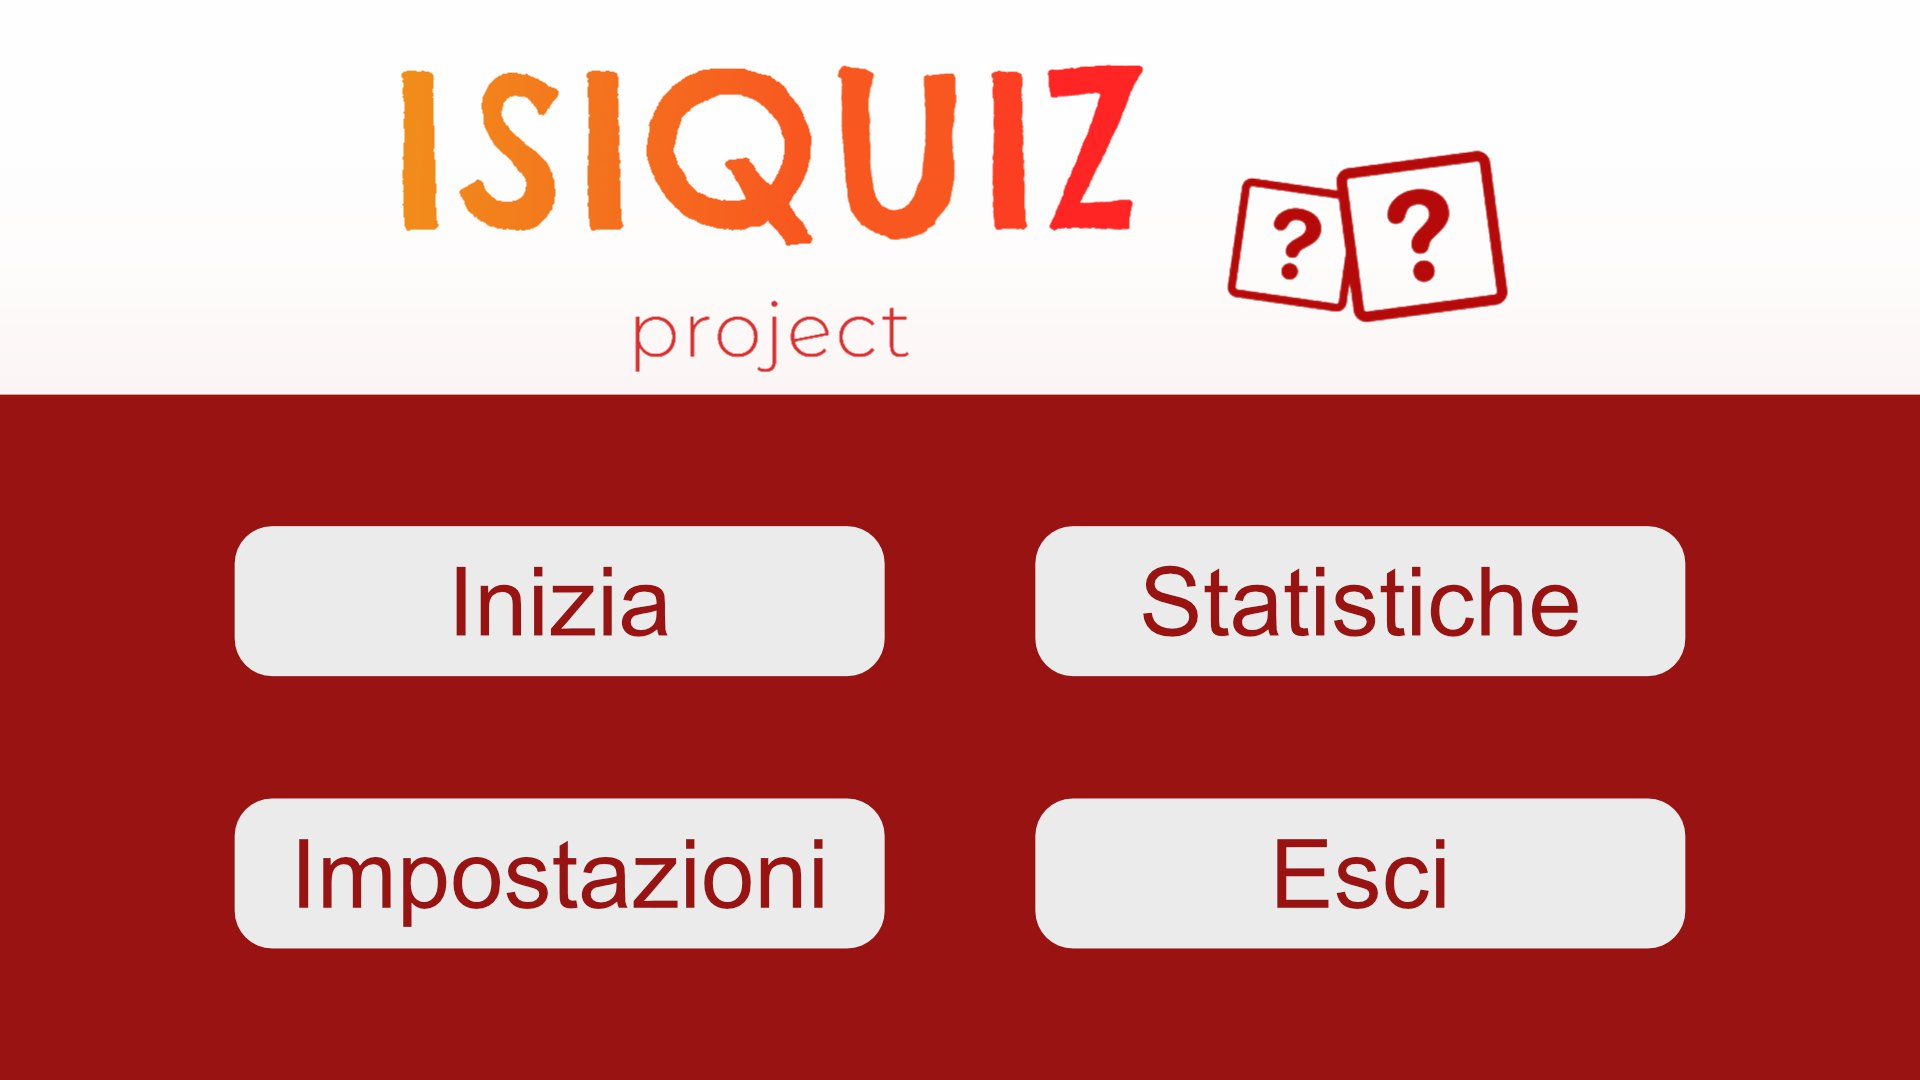
\includegraphics[width=\textwidth]{Images/mockup/home1.jpg}
            \caption{Pagina Iniziale}
            \label{fig:HomePage1}
          \end{minipage}
          \hfill
          \begin{minipage}[b]{0.48\textwidth}
            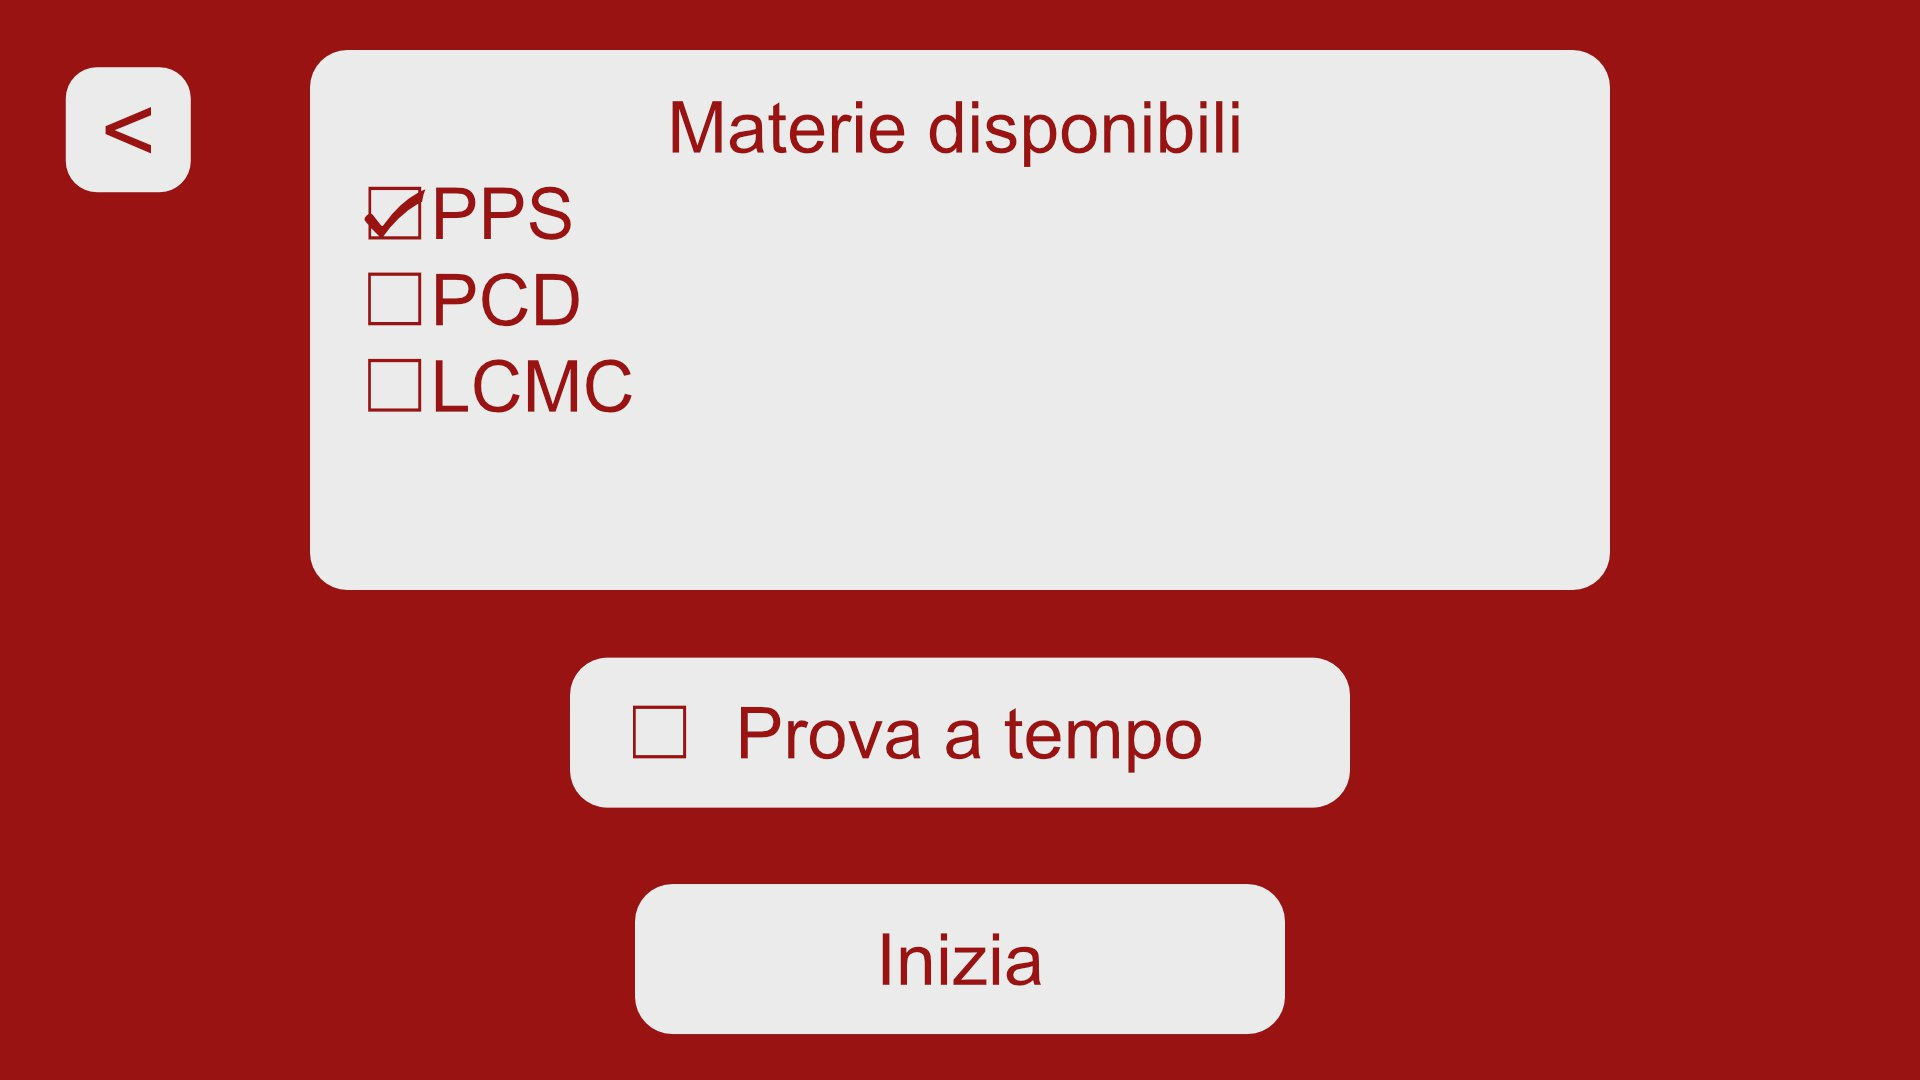
\includegraphics[width=\textwidth]{Images/mockup/start1.jpg}
            \caption{Settaggio di una partita prima di iniziarla}
            \label{fig:Start1}
          \end{minipage}
        \end{figure}

        \begin{figure}[H]
          \centering
          \begin{minipage}[b]{0.48\textwidth}
            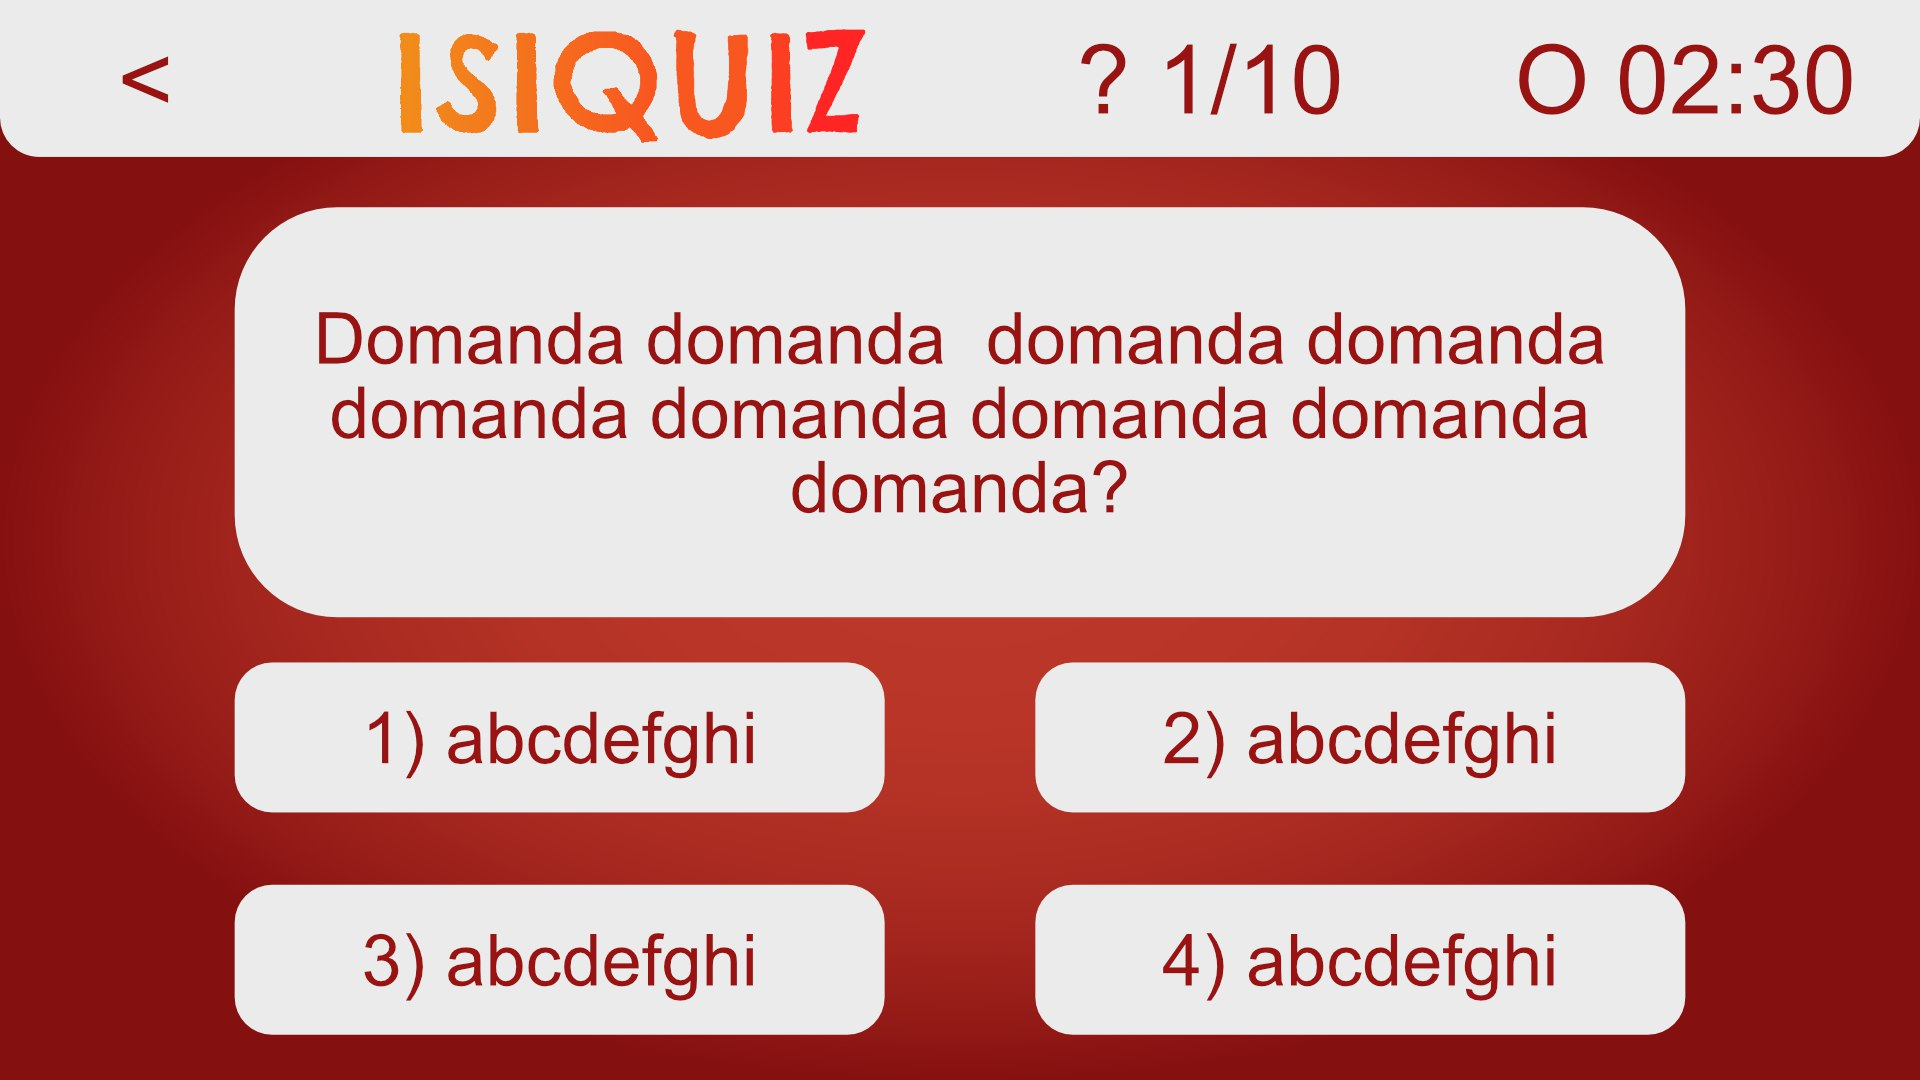
\includegraphics[width=\textwidth]{Images/mockup/quiz1.jpg}
            \caption{Quiz}
            \label{fig:Quiz1}
          \end{minipage}
          \hfill
          \begin{minipage}[b]{0.48\textwidth}
            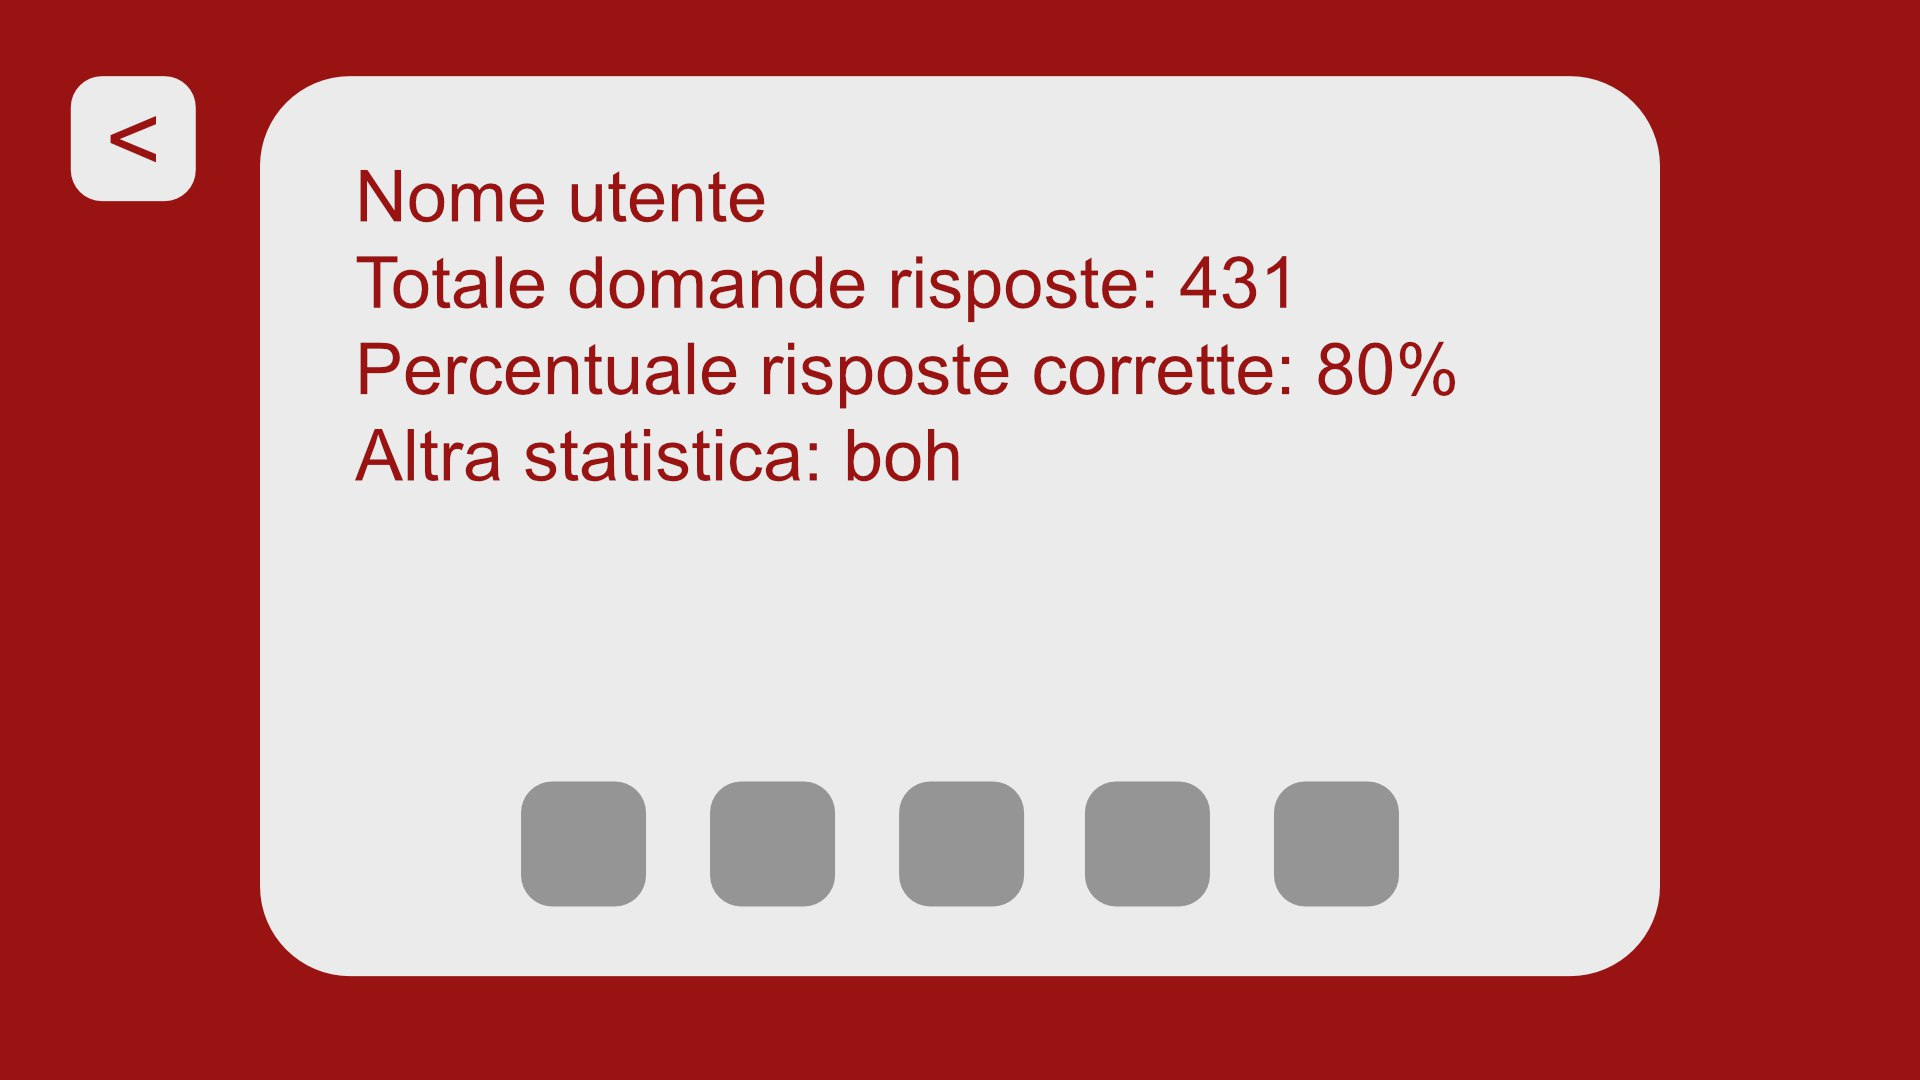
\includegraphics[width=\textwidth]{Images/mockup/achievements1.jpg}
            \caption{Statistiche di gioco e obiettivi raggiunti}
          \end{minipage}
        \end{figure}
          
        \begin{figure}[H]
          \centering
          \begin{minipage}[b]{0.48\textwidth}
            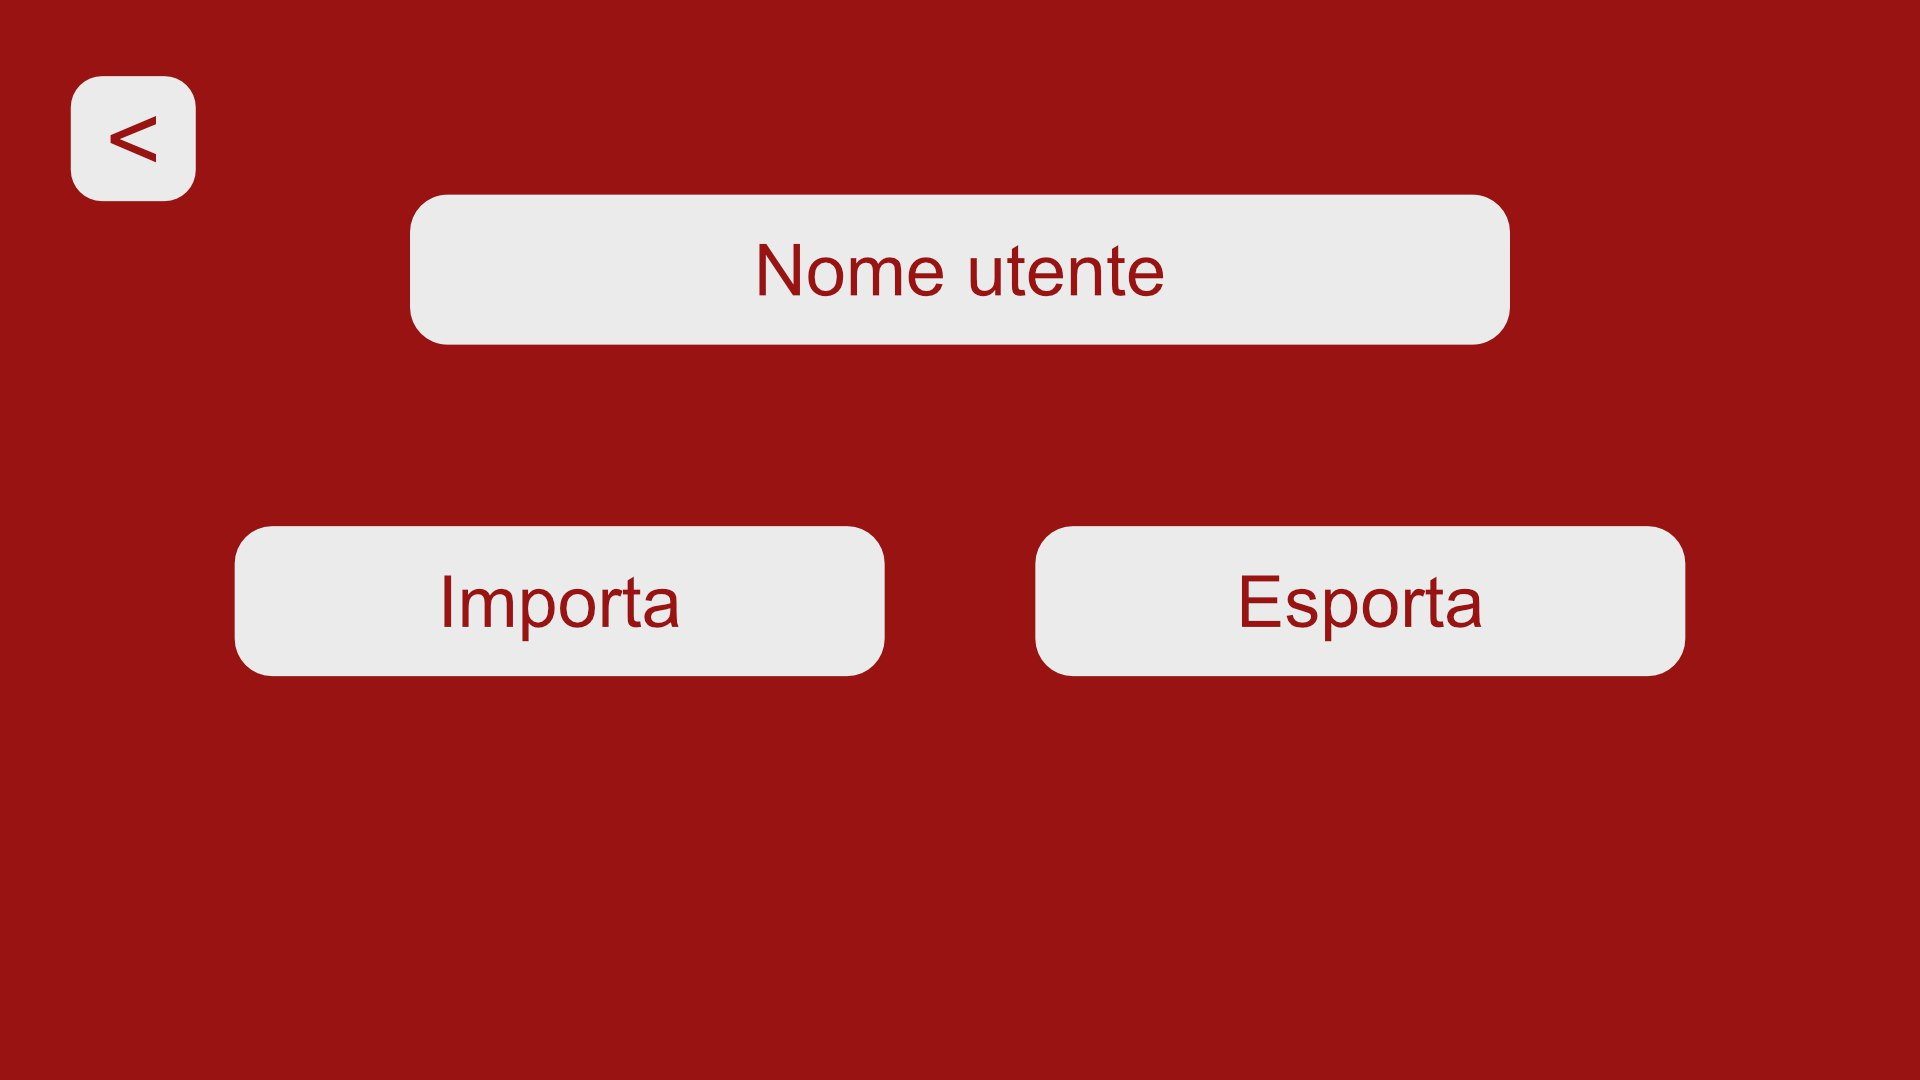
\includegraphics[width=\textwidth]{Images/mockup/settings1.jpg}
            \caption{Impostazioni Generali}
            \label{fig:Settings1}
          \end{minipage}
          \hfill
        \end{figure}
        
        \subsubsection{Mockup seconda versione}\label{mockup2}
        
        \begin{figure}[H]
          \centering
          \begin{minipage}[b]{0.48\textwidth}
            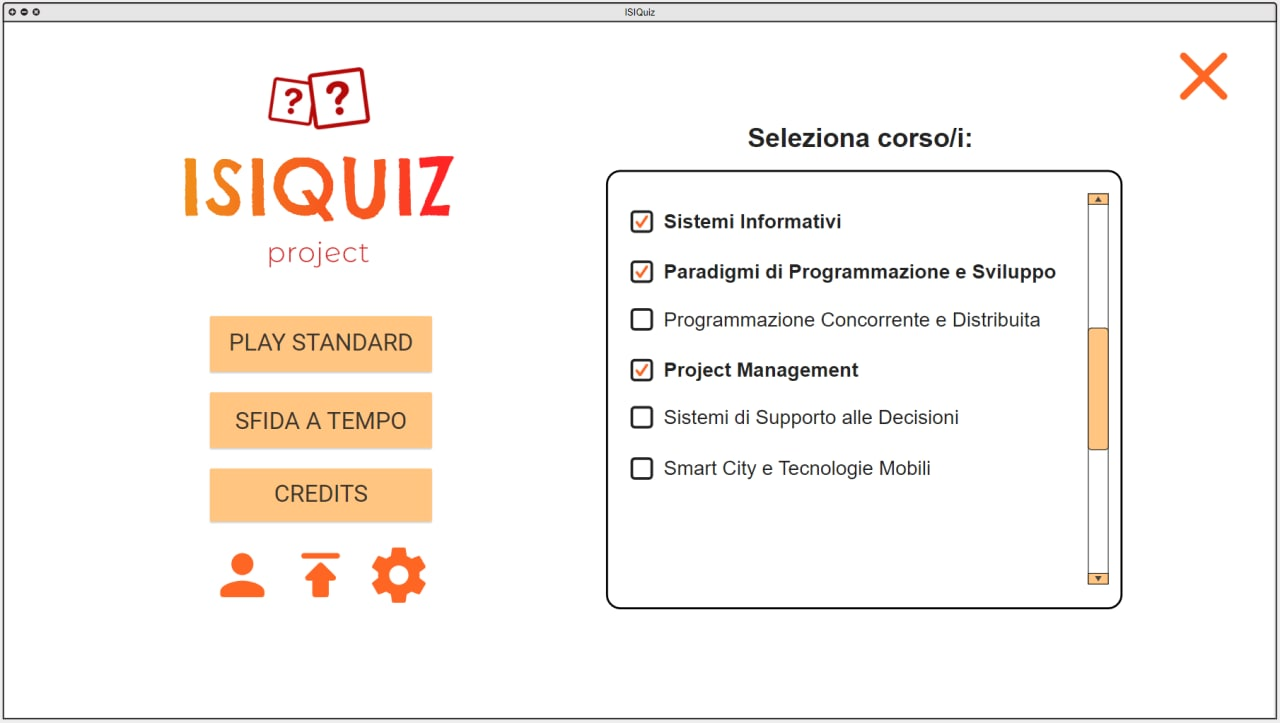
\includegraphics[width=\textwidth]{Images/mockup/home2.jpg}
            \caption{Pagina Iniziale}
            \label{fig:HomePage2}
          \end{minipage}
          \hfill
          \begin{minipage}[b]{0.48\textwidth}
            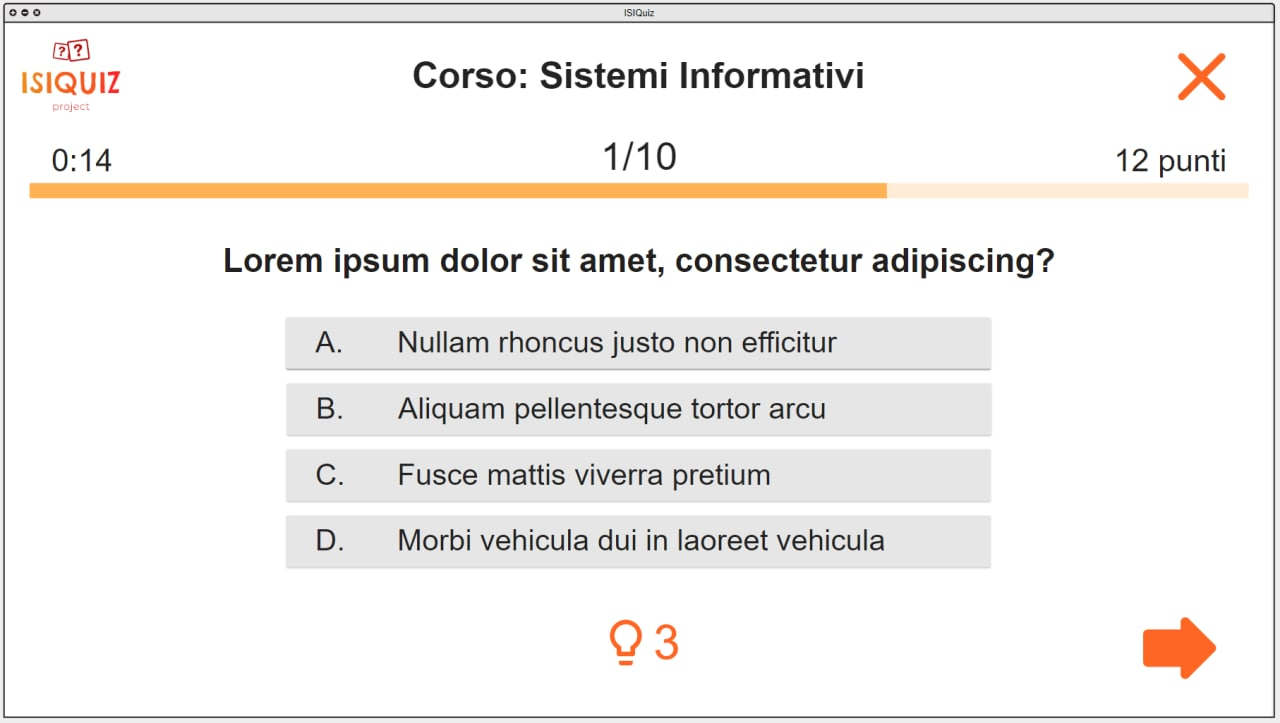
\includegraphics[width=\textwidth]{Images/mockup/quiz2.jpg}
            \caption{Quiz}
            \label{fig:Quiz2}
          \end{minipage}
        \end{figure}
          
        \begin{figure}[H]
          \centering
          \begin{minipage}[b]{0.48\textwidth}
            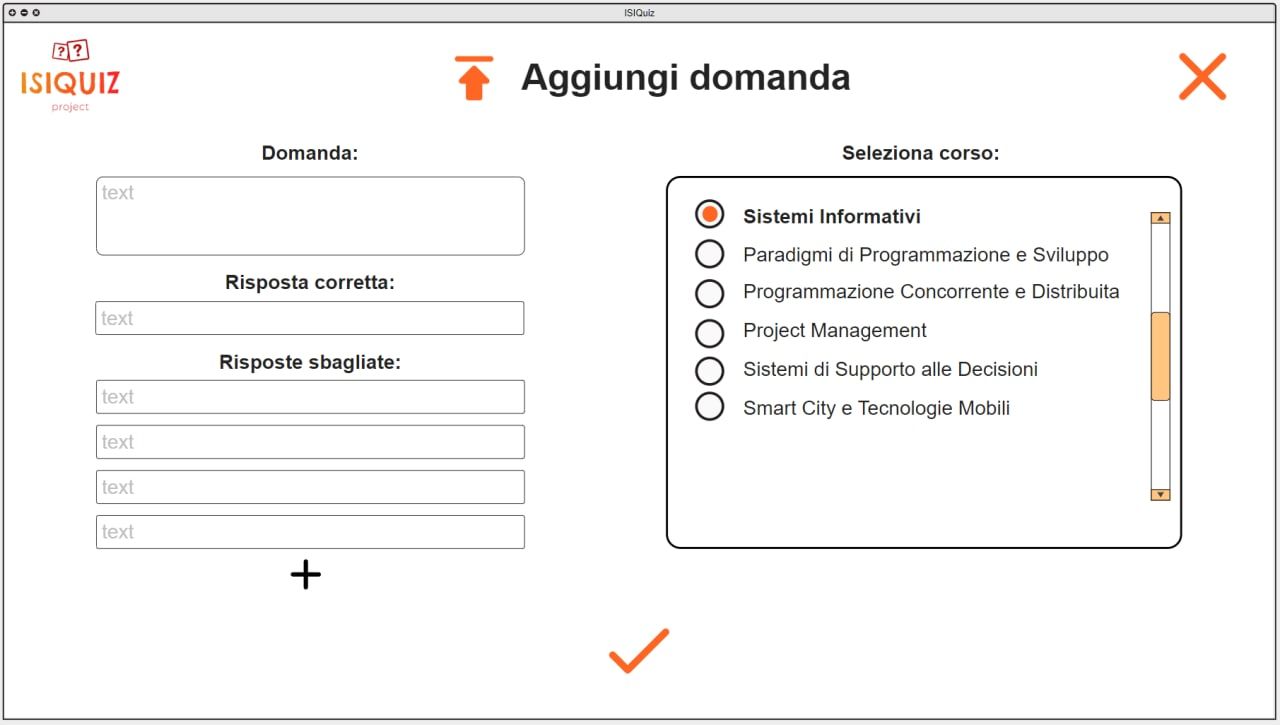
\includegraphics[width=\textwidth]{Images/mockup/import2.jpg}
            \caption{Inserimento di nuove domande e relative risposte per un determinato corso}
            \label{fig:Import2}
          \end{minipage}
          \hfill
        \end{figure}
        
        \subsubsection{Mockup definitivi}\label{mockupFinished}
        
        \begin{figure}[H]
          \centering
          \begin{minipage}[b]{0.48\textwidth}
            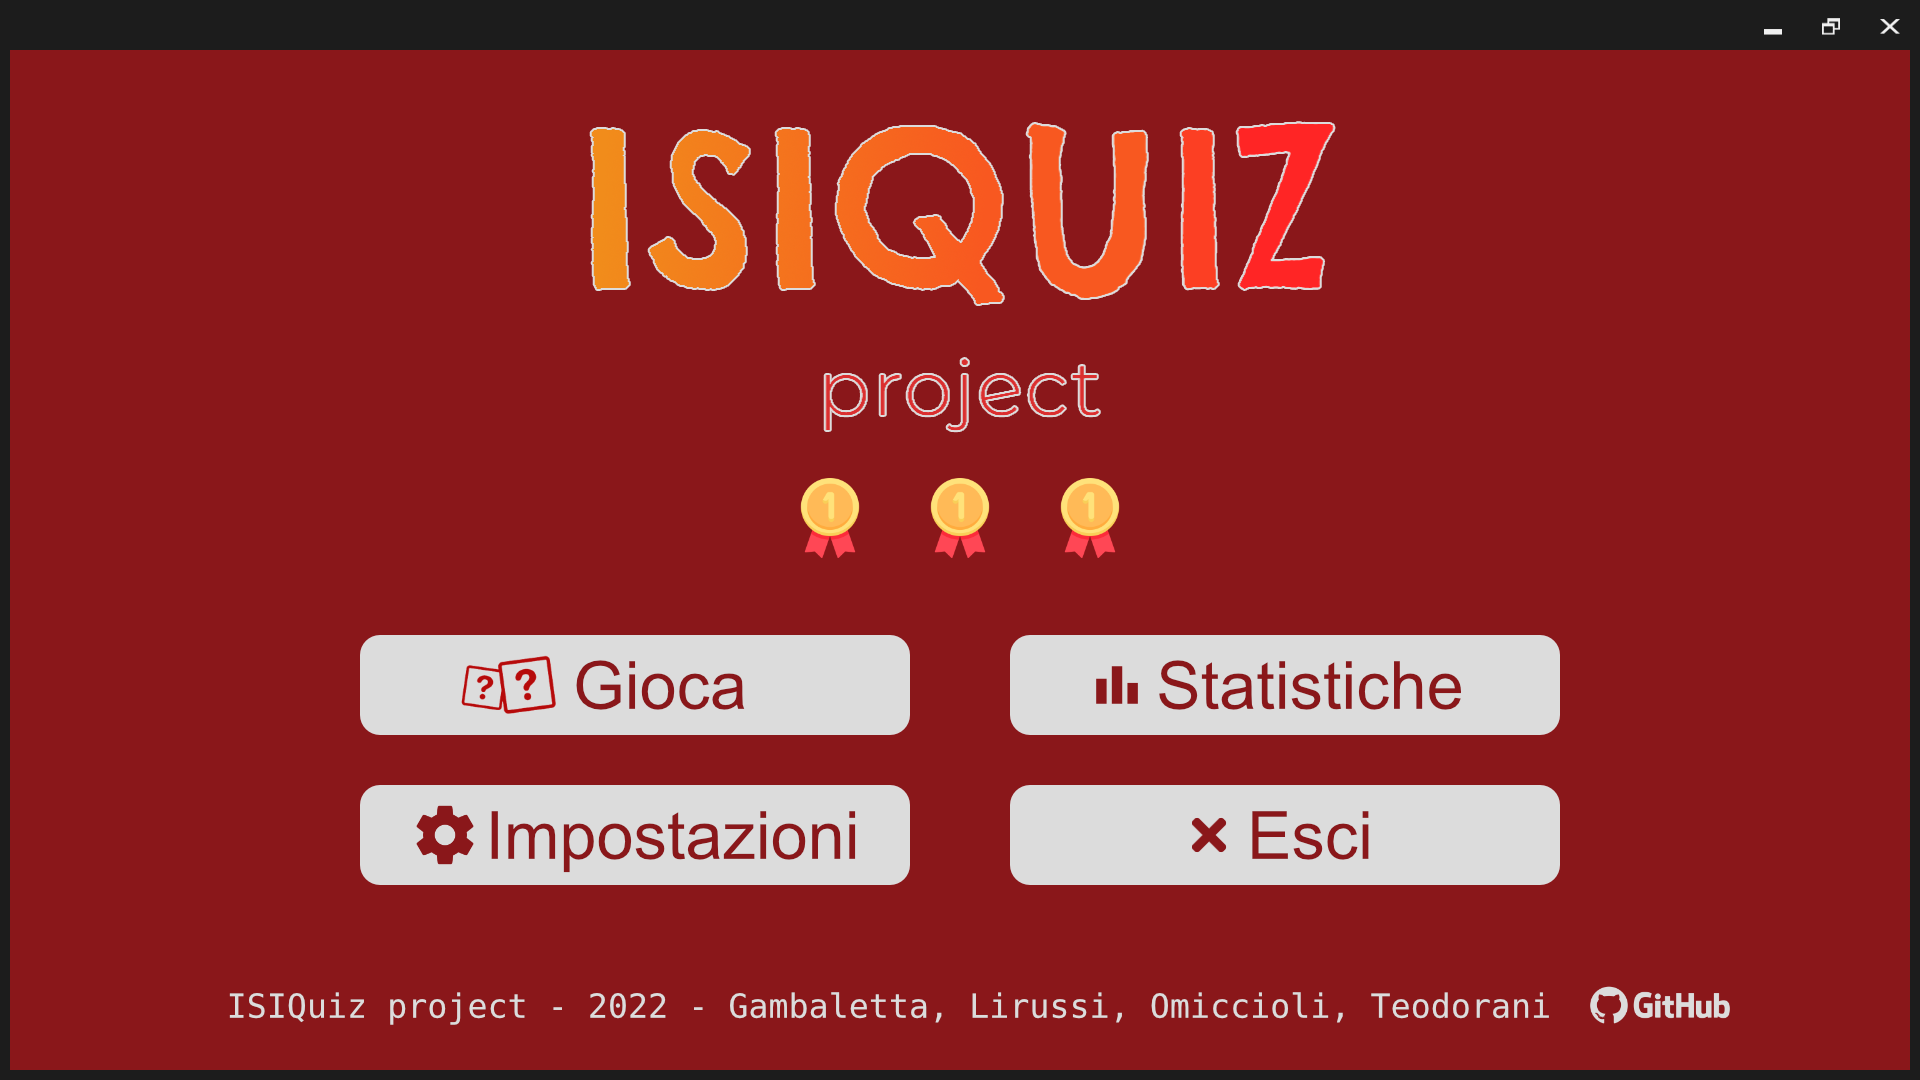
\includegraphics[width=\textwidth]{Images/mockup/home3.png}
            \caption{Pagina iniziale}
            \label{fig:home3}
          \end{minipage}
          \hfill
          \begin{minipage}[b]{0.48\textwidth}
            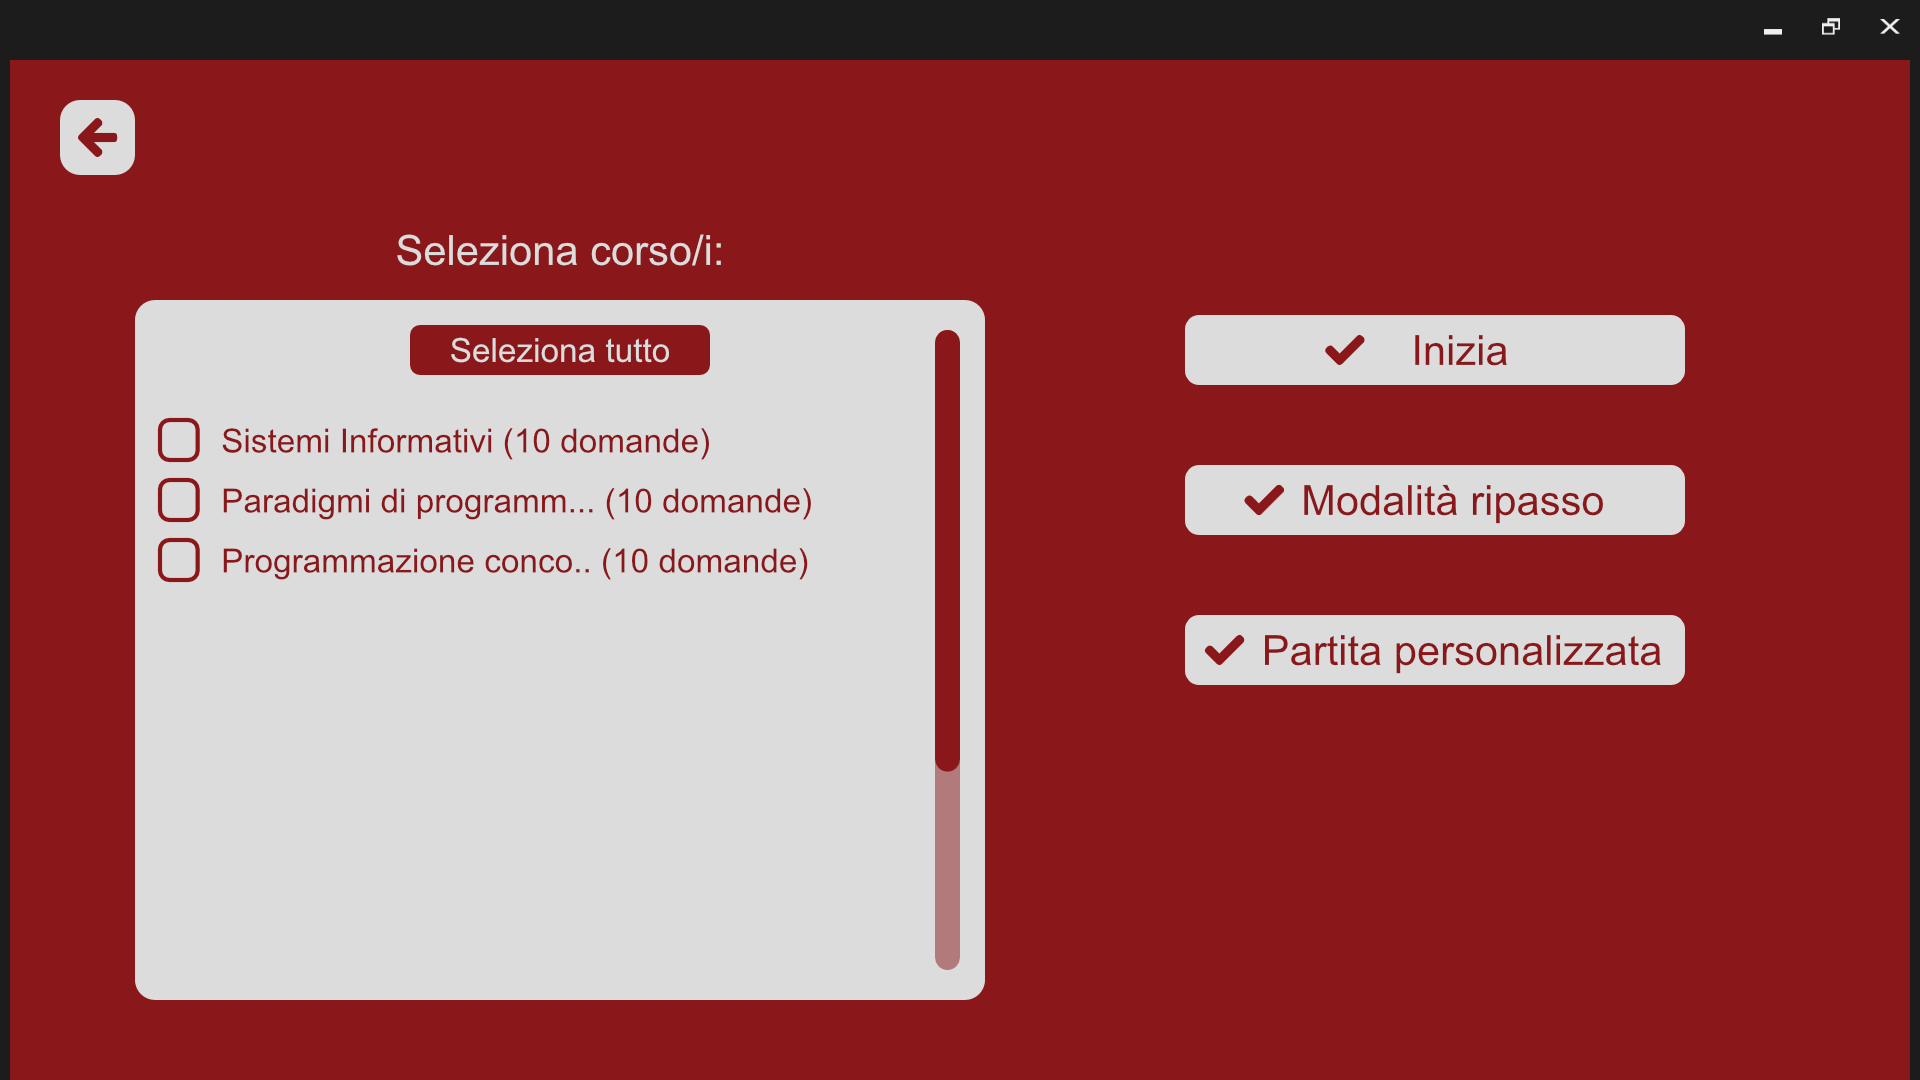
\includegraphics[width=\textwidth]{Images/mockup/start3.png}
            \caption{Settaggio di una partita prima di iniziarla}
            \label{fig:start3}
          \end{minipage}
        \end{figure}

        \begin{figure}[H]
          \centering
          \begin{minipage}[b]{0.48\textwidth}
            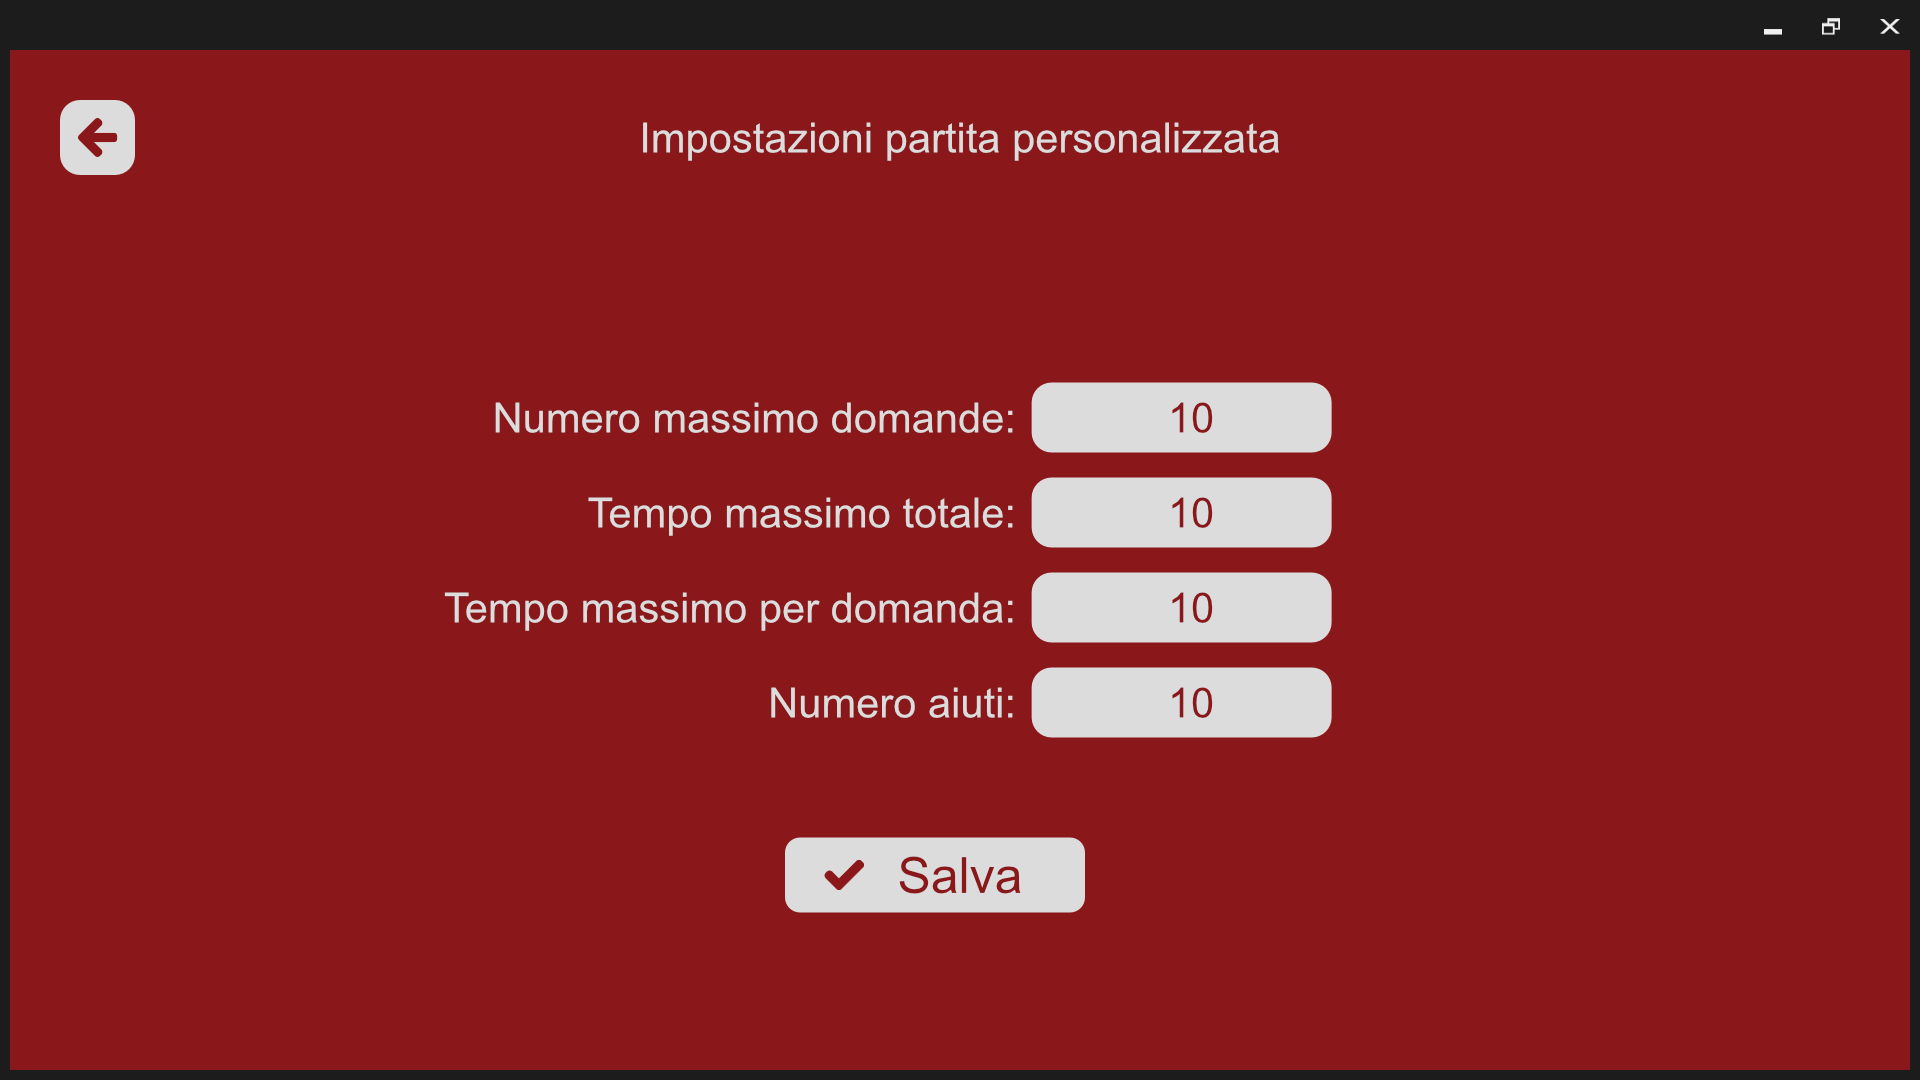
\includegraphics[width=\textwidth]{Images/mockup/custom.png}
            \caption{Settaggio parametri per una partita personalizzata}
            \label{fig:custom}
          \end{minipage}
          \hfill
          \begin{minipage}[b]{0.48\textwidth}
            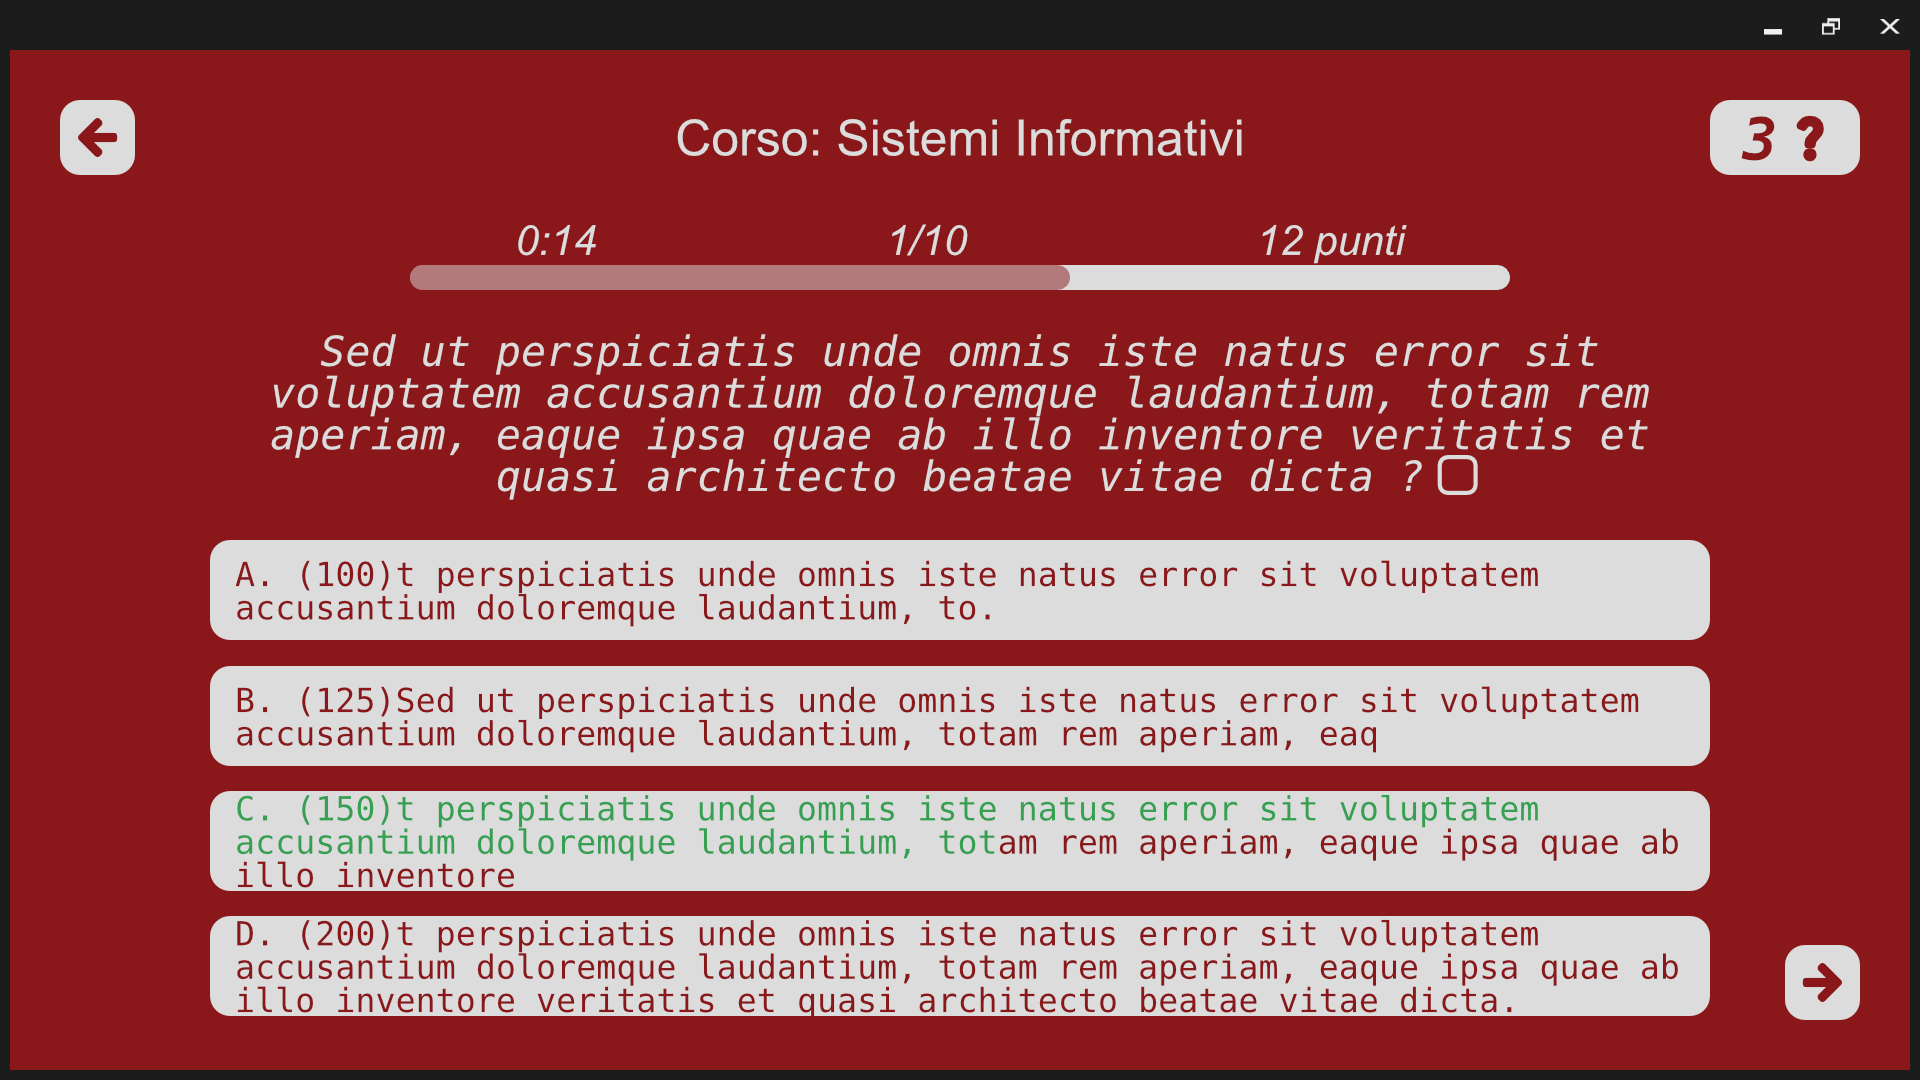
\includegraphics[width=\textwidth]{Images/mockup/quiz3.png}
            \caption{Quiz}
            \label{fig:quiz3}
          \end{minipage}
        \end{figure}

        \begin{figure}[H]
          \centering
          \begin{minipage}[b]{0.48\textwidth}
             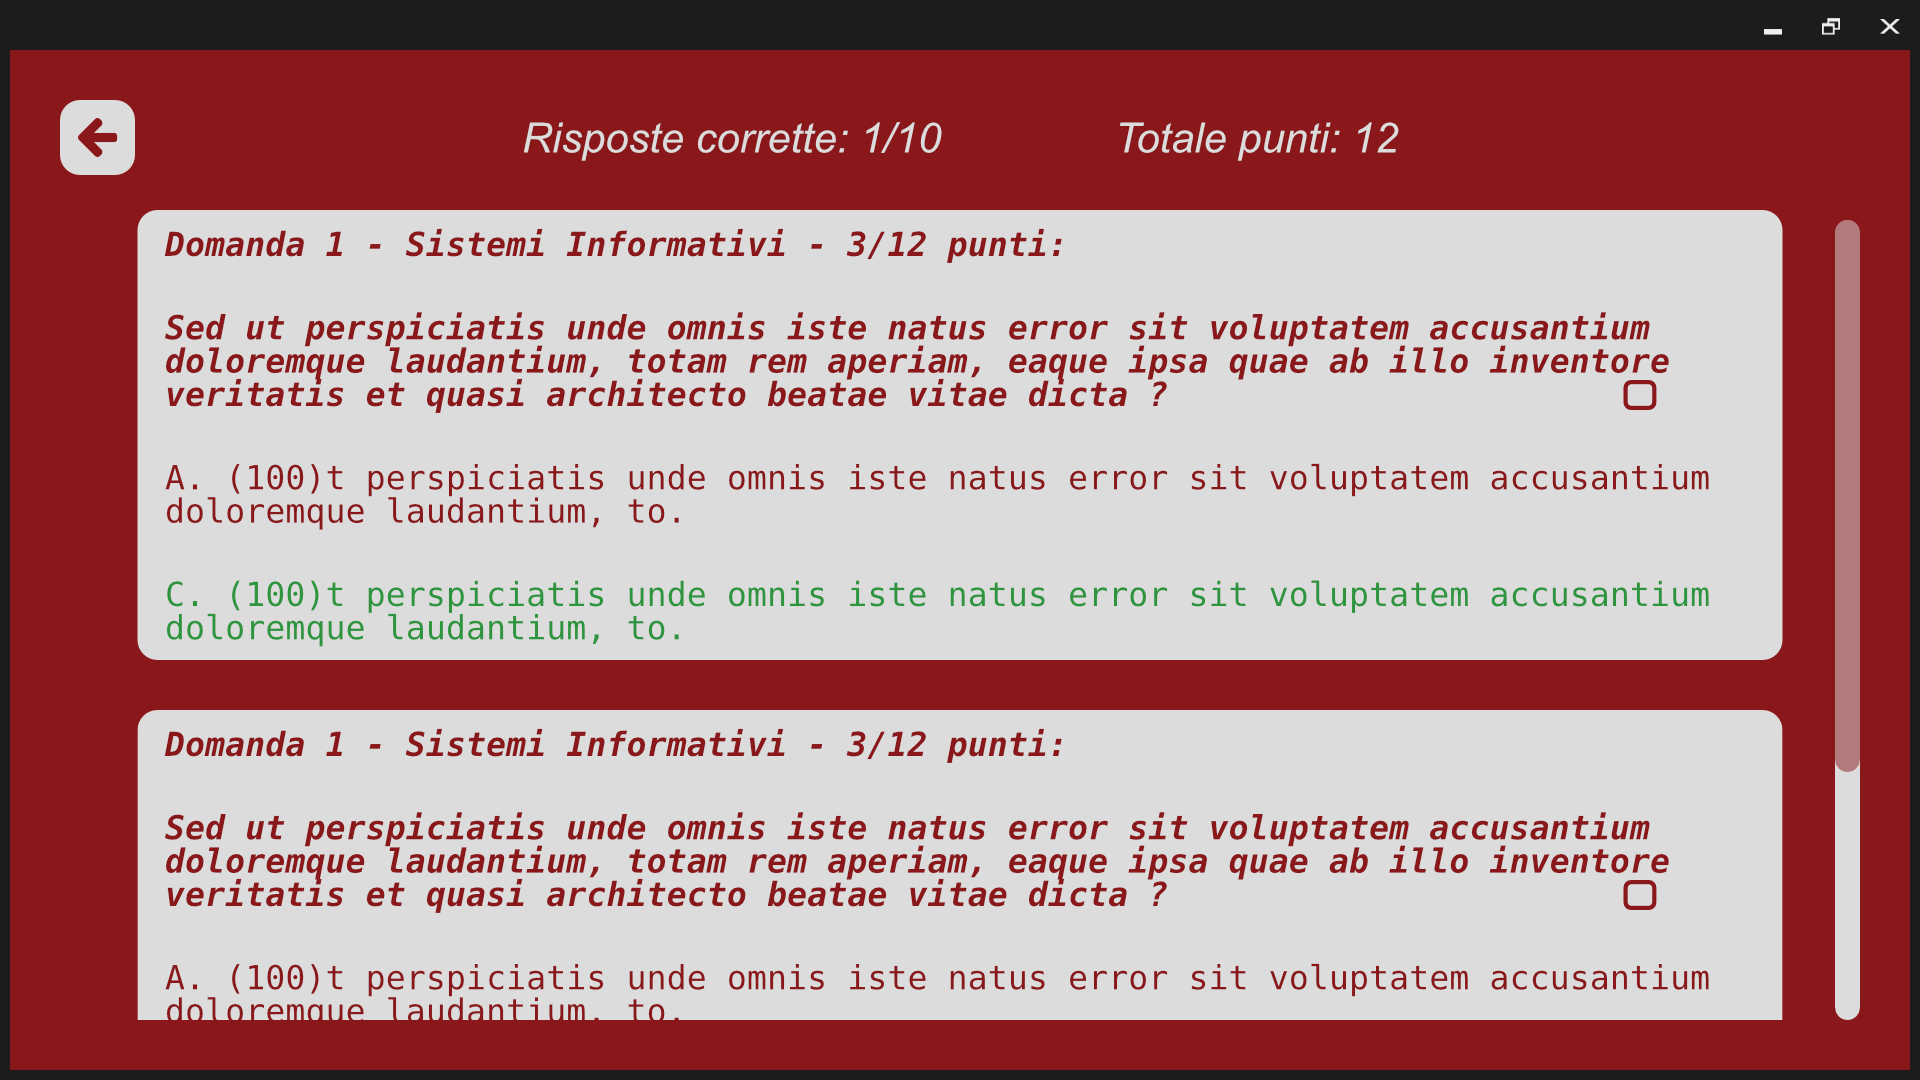
\includegraphics[width=\textwidth]{Images/mockup/review.png}
            \caption{Riepilogo al termine di un quiz}
            \label{fig:review}
          \end{minipage}
          \hfill
          \begin{minipage}[b]{0.48\textwidth}
            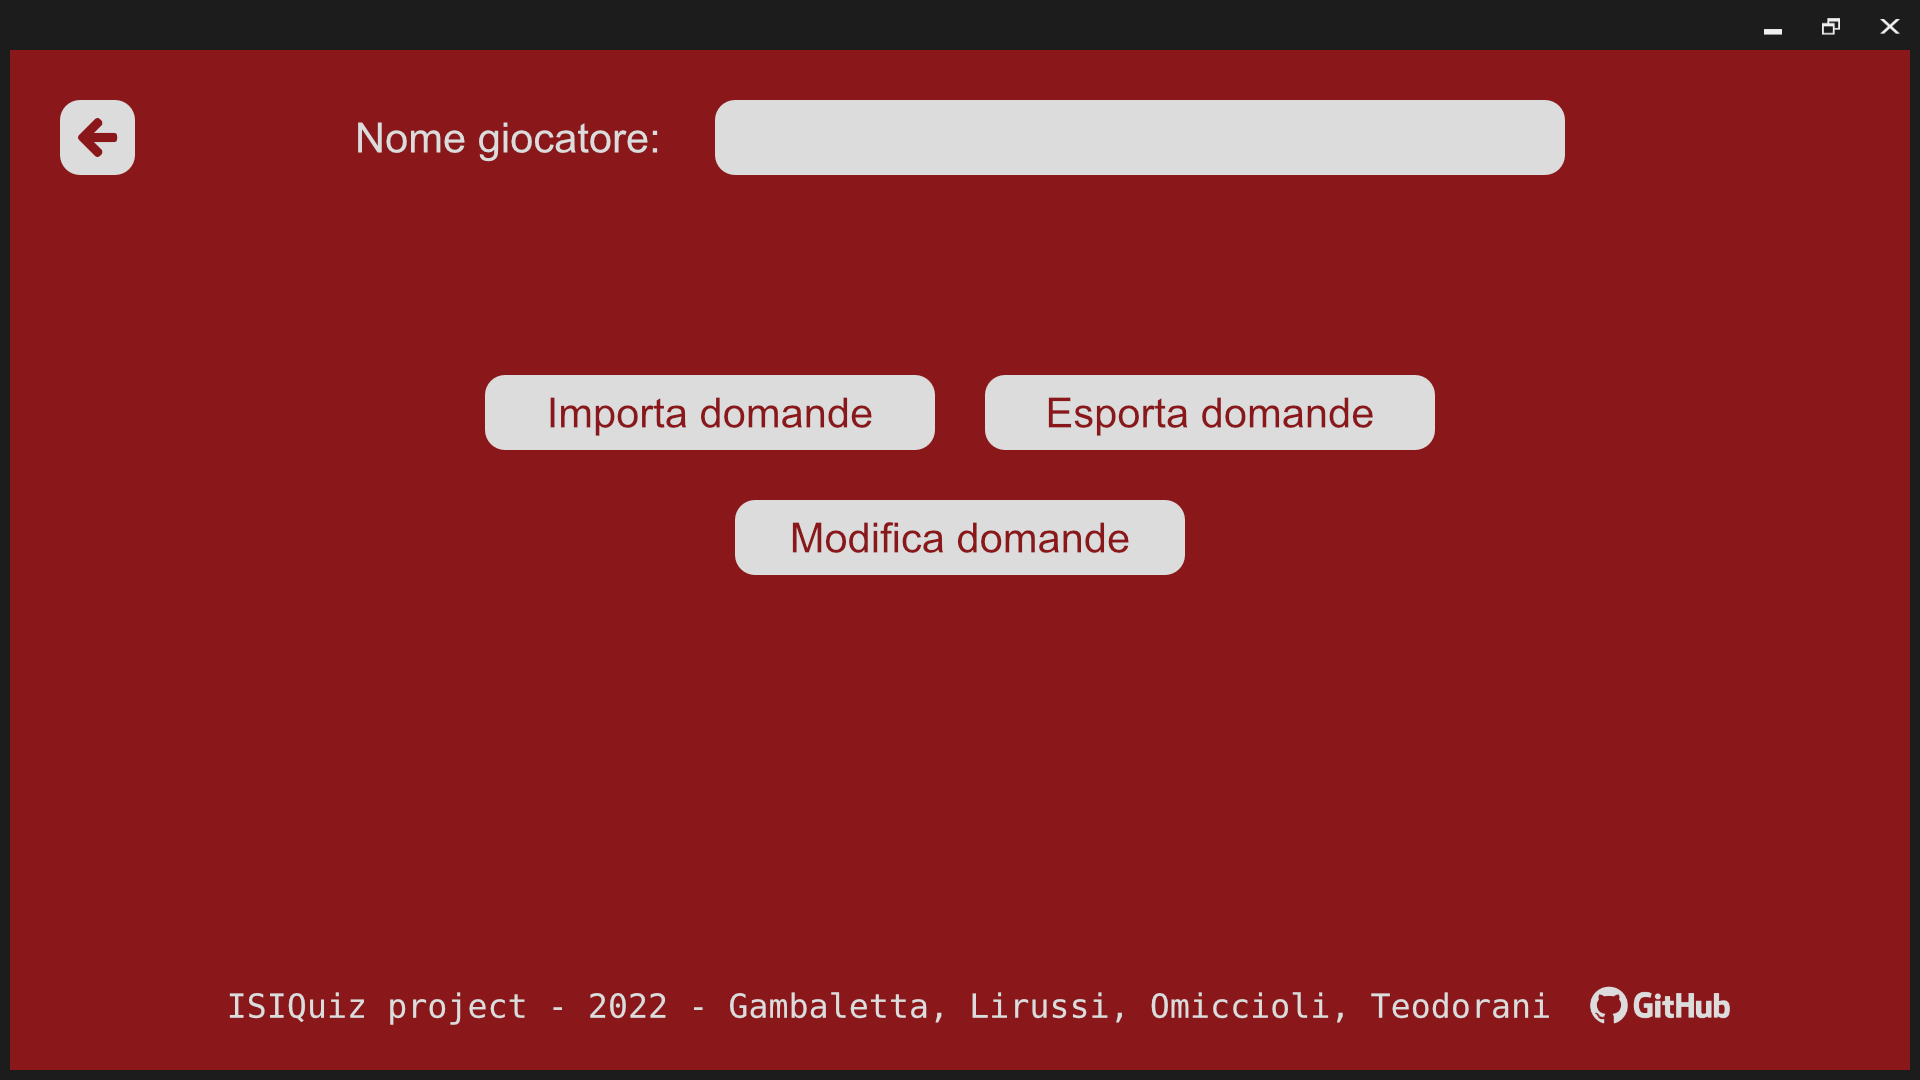
\includegraphics[width=\textwidth]{Images/mockup/settings3.png}
            \caption{Impostazioni generali}
            \label{fig:settings3}
          \end{minipage}
        \end{figure}

        \begin{figure}[H]
          \centering
          \begin{minipage}[b]{0.48\textwidth}
            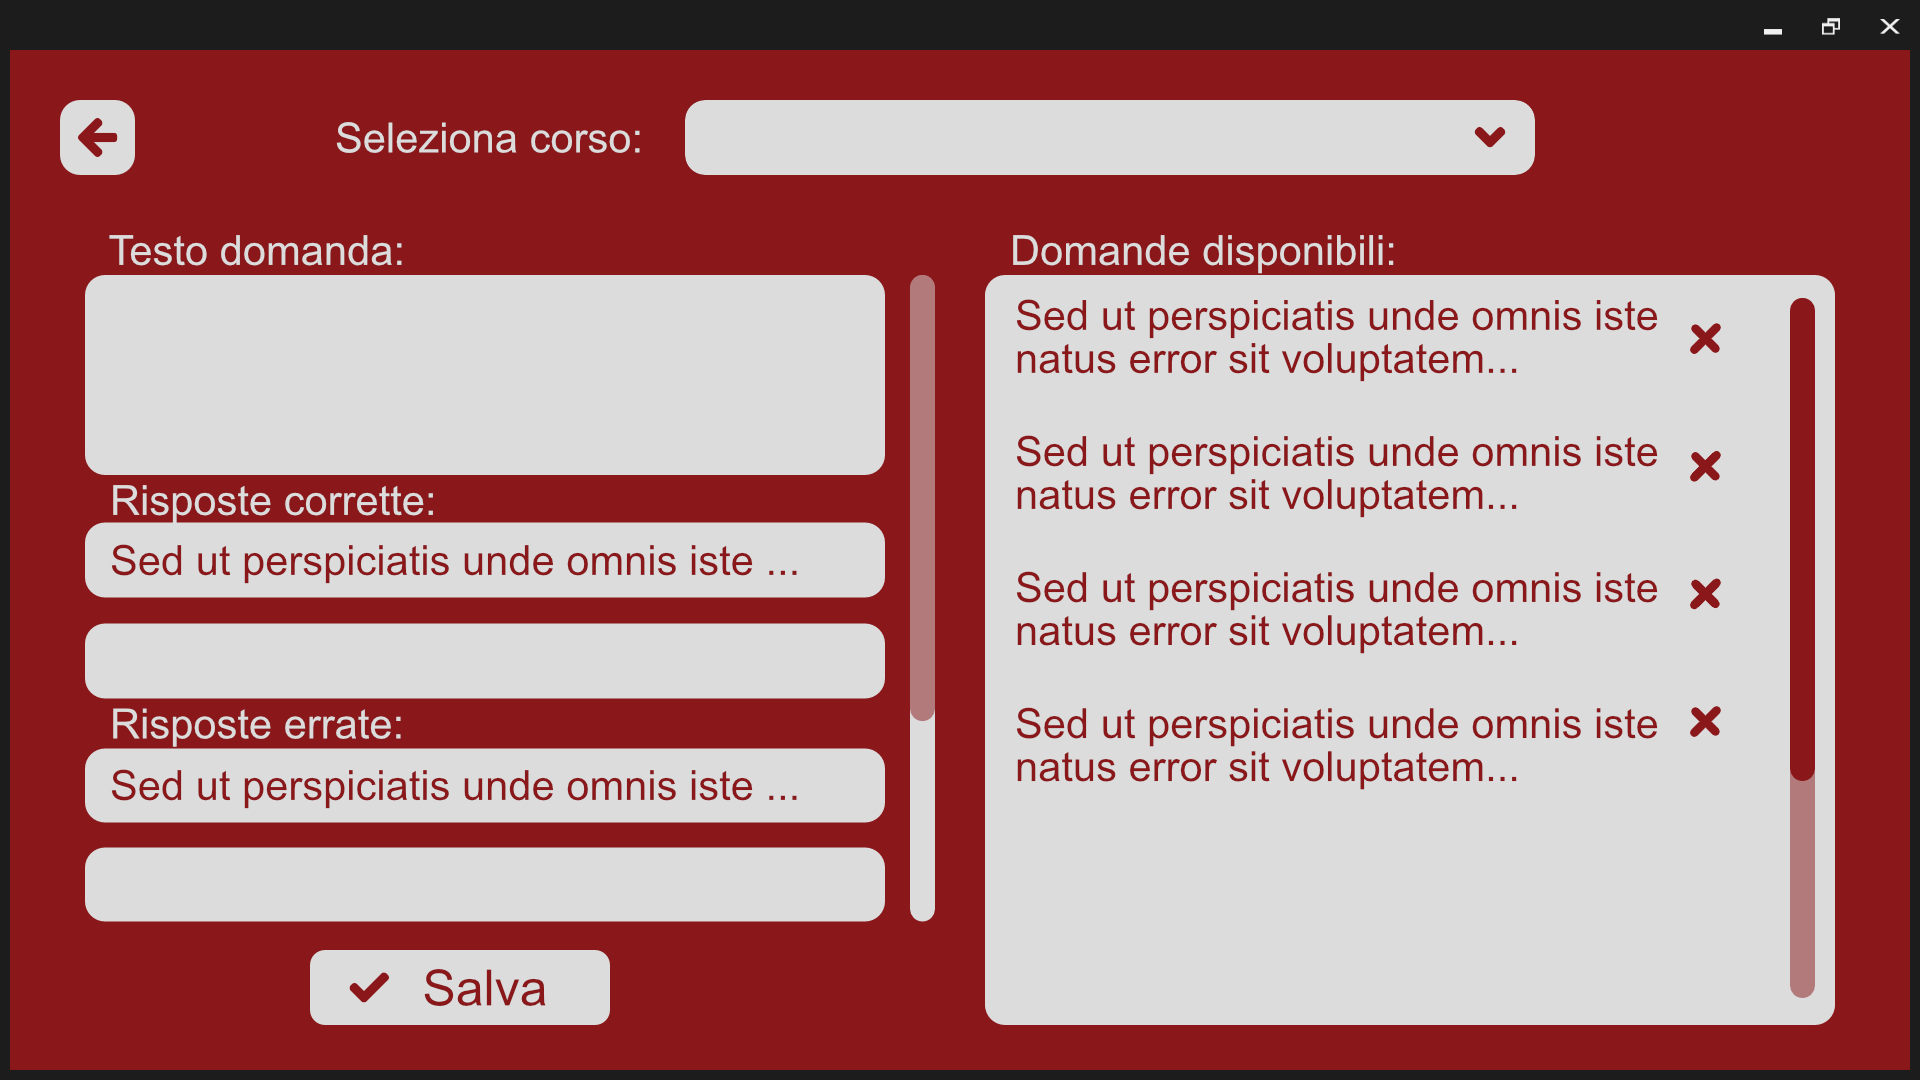
\includegraphics[width=\textwidth]{Images/mockup/import3.png}
            \caption{Inserimento di nuove domande e relative risposte per un determinato corso}
            \label{fig:import3}
          \end{minipage}
          \hfill
          \begin{minipage}[b]{0.48\textwidth}
            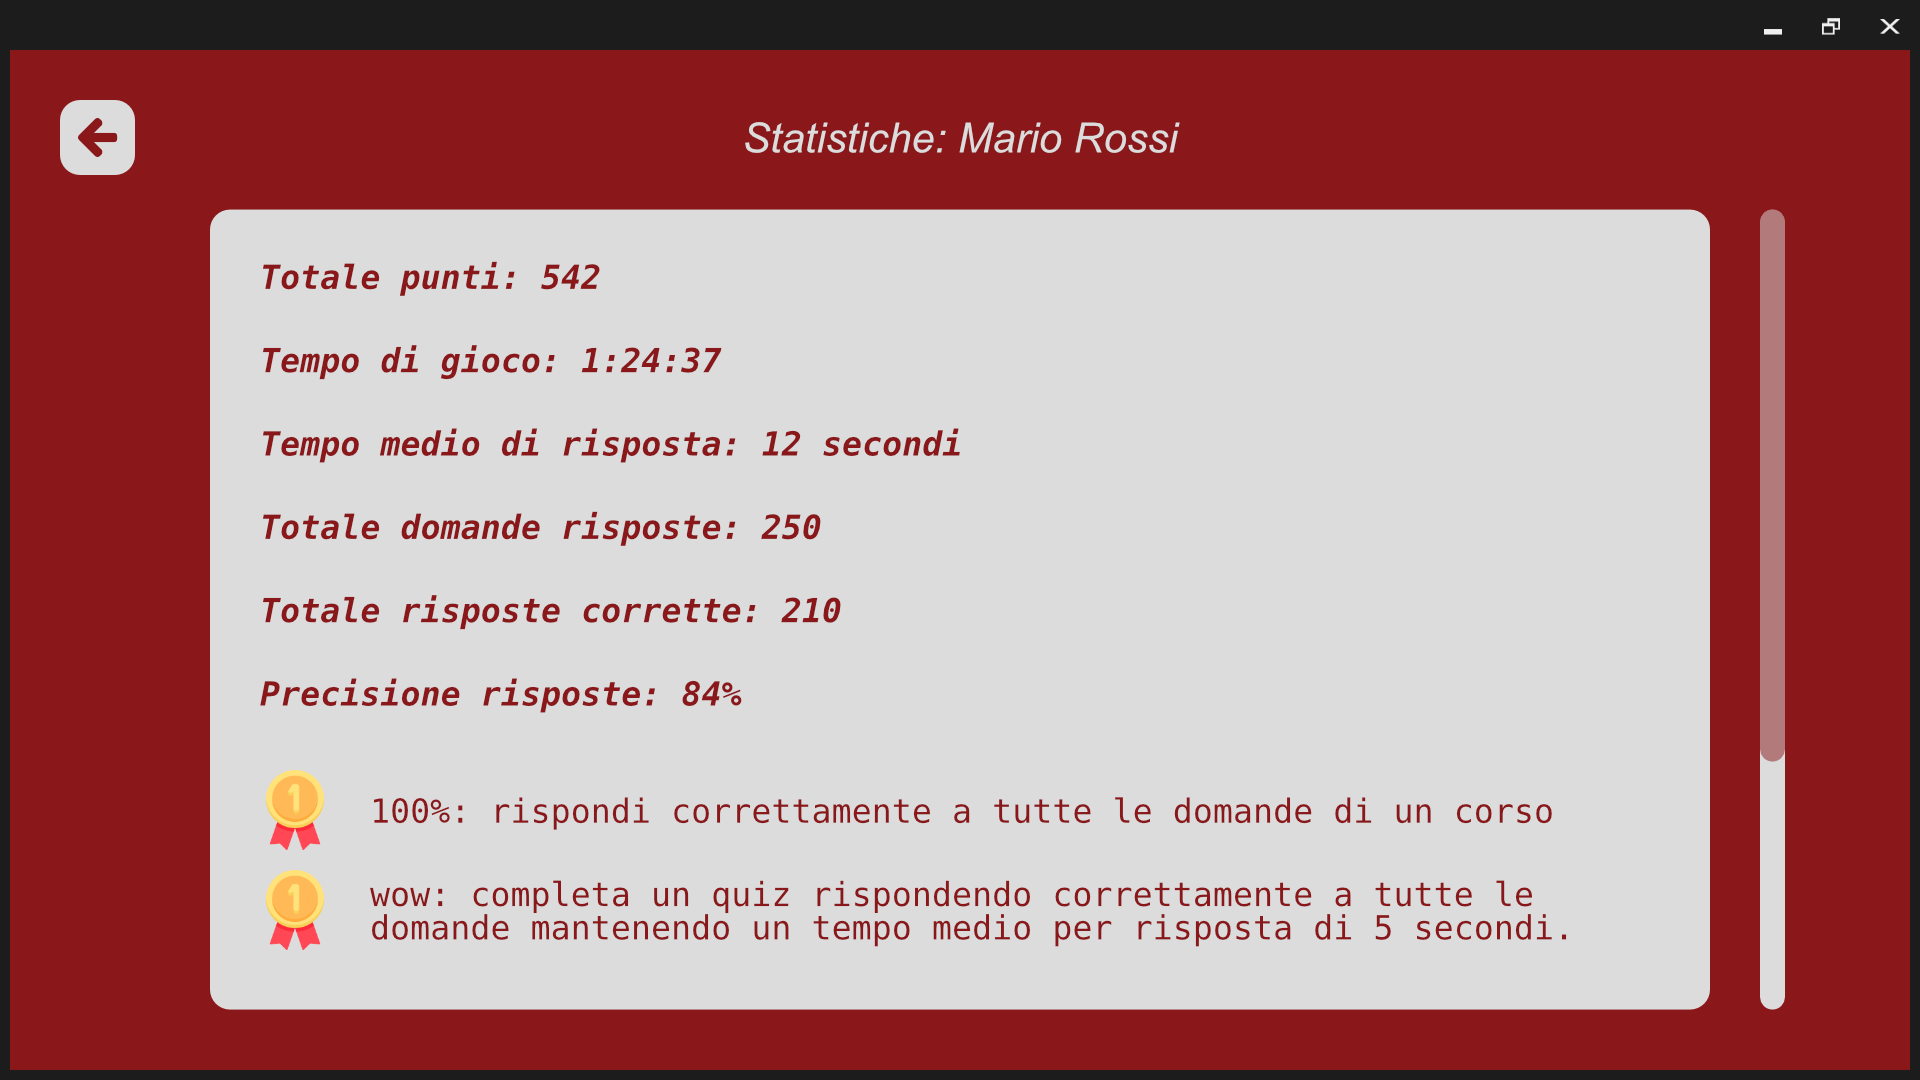
\includegraphics[width=\textwidth]{Images/mockup/achievements3.png}
            \caption{Statistiche di gioco e obiettivi raggiunti}
            \label{fig:achievements3}
          \end{minipage}
        \end{figure}

        \begin{figure}[H]
            \centering
            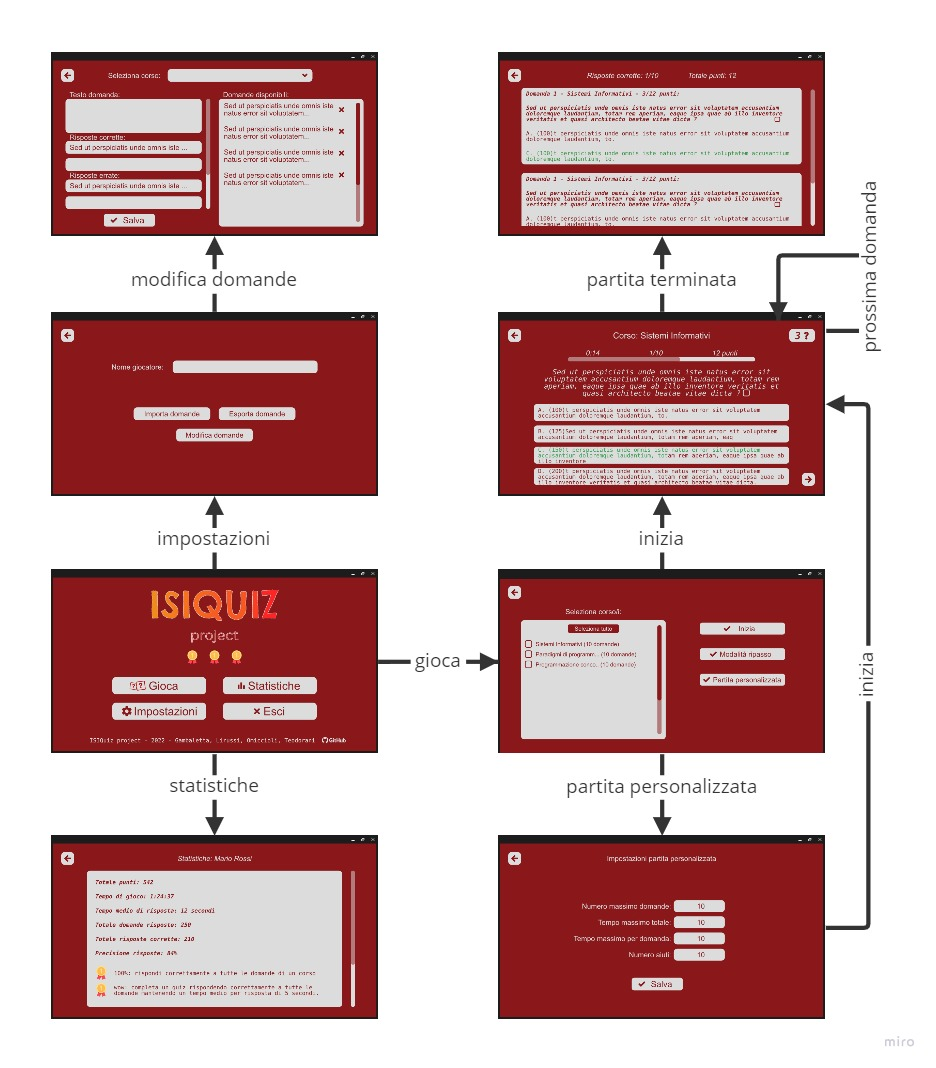
\includegraphics[width=\textwidth]{Miro/mockup_navigation.jpg}
            \caption{Tutti i mockup dell'applicazione con navigazione tra le pagine}
            \label{fig:mockup_nav}
        \end{figure}
	    
\section{Requisiti Funzionali} 
        \subsection{Obbligatori} \label{chap:req_funzionali}
        All’interno di ogni partita, vengono presentate all’utente diverse domande di natura accademica, ognuna delle quali viene accompagnata da un numero predeterminato di risposte possibili, alcune corrette ed altre sbagliate. L’utente dovrà individuare le risposte corrette in un tempo massimo per non fallire la domanda. 

        \begin{enumerate}
            \item \textbf{Modalità di gioco standard}: domande a scelta multipla su tutti i corsi disponibili: al giocatore verranno posti dieci quiz scelti casualmente tra tutti i corsi disponibili nel gioco. Ogni domanda dovrà essere risposta in massimo quindici secondi altrimenti verrà considerata errata.
            
            \item \textbf{Modalità di gioco materie a scelta}: domande a scelta multipla su alcuni dei corsi scelti dal giocatore tra tutti i corsi disponibili: al giocatore verranno posti dieci quiz scelti casualmente tra tutti i corsi selezionati. Ogni domanda dovrà essere risposta in massimo quindici secondi altrimenti verrà considerata errata.
            
            \item \textbf{Modalità di gioco materia specifica}: domande a scelta multipla su un corso scelto dal giocatore tra tutti i corsi disponibili: al giocatore verranno posti dieci quiz scelti casualmente tra quelli disponibili per il corso specificato. Ogni domanda dovrà essere risposta in massimo quindici secondi altrimenti verrà considerata errata.

            \item \textbf{Modalità di gioco personalizzata}: domande a scelta multipla su alcuni dei corsi scelti dal giocatore tra tutti i corsi disponibili: prima dell'inizio della partita il giocatore può decidere a quanti quiz rispondere (N) e il tempo massimo (T) in cui rispondere a ciascun quiz. Al giocatore verranno quindi posti N quiz scelti casualmente tra tutti i corsi selezionati. Ogni domanda dovrà essere risposta in T tempo massimo altrimenti verrà considerata errata.

            \item \textbf{Interfaccia grafica} (CLI e successivamente ScalaFX): visualizzazione menu principale, visualizzazione della domanda e di quattro possibili risposte da scegliere durante il gioco, visualizzazione dei risultati post partita. La prima iterazione del programma dovrà fornire una semplice interfaccia da terminale che permetta di interagire con le funzionalità principali del gioco scrivendo le operazioni da eseguire tramite linea di comando. Successivamente verrà sostituita da una GUI.
                \begin{enumerate}
                    \item Menu principale: la prima pagina che verrà mostrata all'avvio
                        \begin{enumerate}
                            \item Pulsante "inizia a giocare" > pagina selezione corsi
                            \item Pulsante "statistiche" > pagina statistiche
                            \item Pulsante "impostazioni" > pagina impostazioni
                            \item Pulsante "esci" > termina l'applicazione
                        \end{enumerate}
                    \item Pagina statistiche: contiene informazioni sulle statistiche relative alle partite concluse
                        \begin{enumerate}
                            \item Totale quiz risposti
                            \item Totale quiz risposti correttamente
                            \item Percentuale risposte corrette
                        \end{enumerate}
                    \item Pagina impostazioni: permette di editare i quiz, cioè le domande e le risposte, oltre a salvarli ed importarli da file
                        \begin{enumerate}
                            \item Modulo per editare i quiz
                            \item Pulsante per salvare (esportare) nuovi quiz > salva su file tutti i quiz dei corsi
                            \item Pulsante per importare nuovi quiz > permette di selezionare un file contenente i corsi con i relativi quiz
                        \end{enumerate}
                    \item Pagina selezione corsi: permette di modificare alcune impostazioni di gioco e di selezionare i corsi dai quali devono essere presi i quiz prima di iniziare la partita
                        \begin{enumerate}
                            \item Selezione corsi disponibili
                            \item Personalizza tempo per risposta
                            \item Personalizza numero domande della partita
                        \end{enumerate}
                    \item Pagina riepilogo post partita: permette di visualizzare il punteggio ottenuto nella partita appena conclusa e la lista di tutti i quiz con un'indicazione sulla correttezza della risposta data e, in caso di risposta errata, la risposta corretta corrispondente
                    \begin{enumerate}
                        \item Testo con punteggio della partita
                        \item Lista quiz della partita con risposta scelta ed eventualmente risposta corretta
                    \end{enumerate}
                \end{enumerate}
            
            \item \textbf{Punteggio finale} del quiz appena effettuato: al termine della partita verrà visualizzato il punteggio ottenuto dal giocatore in base al numero di risposte corrette o errate date nella partita conclusa. il punteggio totale della partita verrà calcolato sommando i punti relativi ad ogni quiz risposto correttamente. Nella modalità di gioco standard, quella in cui ogni quiz ha un tempo massimo di risposta, il punteggio associato ad ognuno viene diminuito man mano che passa il tempo a disposizione.
            
            \item \textbf{Visualizzazione e salvataggio delle statistiche personali}: in specifico le statistiche personali includono:
                \begin{enumerate}
                    \item Totale dei quiz risposti
                    \item Totale risposte corrette
                    \item Percentuale di correttezza delle risposte
                    \item Punteggio totale
                \end{enumerate}
            
            \item \textbf{Più risposte giuste} e sbagliate per ogni domanda in modo da avere una rotazione tra le possibili scelte: ogni domanda dovrà necessariamente avere almeno tre risposte errate ed una corretta, ma potrebbe averne a disposizione un numero superiore, da scegliere poi casualmente durante il gioco. In ogni caso, dovrà essere rispettato il vincolo di avere tre risposte errate ed una corretta per ogni quiz durante la partita.
            
            \item Aggiunta di \textbf{nuovi quiz} con le relative domanda e risposte da parte dell’utente:
                \begin{enumerate}
                        \item Aggiunta di un nuovo corso
                        \item Aggiunta di un nuovo quiz
                        \item Aggiunta di una domanda relativa al nuovo quiz
                        \item Aggiunta di tre o più risposte errate relative ad un quiz
                        \item Aggiunta di una o più risposta corretta relativa ad un quiz
                        \item Aggiunta di un punteggio per un quiz
                    \end{enumerate}
        \end{enumerate}  

    
        \subsection{Opzionali} \label{chap:req_non_funzionali}
        \begin{enumerate}
            \item \textbf{Sfida a tempo}: rispondere a più domande possibili in un intervallo di tempo limitato
            \item \textbf{Aiuti su richiesta}: all’utente vengono messi a disposizione un numero specifico di aiuti ad ogni partita con i quali semplificare la scelta della risposta. Utilizzando uno degli aiuti verrà eliminata una tra le risposte errate, semplificando così la scelta. Potranno essere utilizzati al massimo due aiuti per ogni domanda
            
            \item \textbf{Revisione solo delle risposte sbagliate}: l’utente può scegliere una modalità di gioco in cui ripassare esclusivamente le domande precedentemente sbagliate
            
            \item \textbf{Medaglie-achievement} quando si completano delle sfide (es. più punti di un certo limite, più giornate continuativamente, aver risposto bene a tutte le domande di una materia)
            
            \item Salvataggio delle statistiche relative al tempo medio di risposta e tempo totale di gioco
        \end{enumerate}
        
	\section{Requisiti Non Funzionali}
        \begin{itemize}
            \item Interfaccia grafica intuitiva e che fornisca feedback coerenti all'utente per comunicargli lo stato delle sue azioni (ad esempio, indicando con colore verde una risposta qualora essa sia corretta)
            \item Interfaccia grafica accessibile agli utenti daltonici
            \item Interfaccia grafica reattiva: alle azioni di un utente devono corrispondere degli aggiornamenti dell'interfaccia stessa in tempi ragionevoli (al massimo un secondo) per non rovinare la user experience
            
            \item Realizzare un sistema modulare che permetta estensioni future (ad esempio, uno sviluppo distribuito che permetta di realizzare funzionalità di gioco multiplayer)
            
            \item Il sistema dovrà essere in grado di memorizzare dati di interesse in maniera consistente
            
            \item Il sistema deve essere funzionante in diversi sistemi operativi nei quali è installata una appropriata Java Virtual Machine (il requisito minimo considera il funzionamento su sistemi Windows, Linux e MacOS)
            
            \item Il sistema deve essere fault-tolerant, cioè deve continuare a funzionare in modo affidabile e deve essere privo di falle che permettano al giocatore di barare
        
        \end{itemize}

\section{Requisiti Implementativi}
        \begin{itemize}
            \item Linguaggio di programmazione Scala versione 3.2.0
            \item Libreria \href{https://openjfx.io}{JavaFX} e il suo wrapper scritto in Scala chiamato \href{https://github.com/scalafx/scalafx}{ScalaFX} per l'interfaccia grafica
            \item Utilizzo di JDK >= 11
            \item Libreria \href{https://github.com/playframework/play-json}{Play JSON} 2.10.0-RC7 per il salvataggio dei quiz e delle statistiche attraverso la notazione JSON.
            \item Per lo sviluppo dovrà essere utilizzato l'IDE IntelliJ in modo da avere consistenza tra i membri del team di sviluppo.
        \end{itemize}

	